% !Mode:: "TeX:UTF-8"
%!TEX program  = xelatex
\documentclass[bwprint]{cumcm}
%===================Package Area==================%
\usepackage{enumitem}
\usepackage{upgreek}
\usepackage{amssymb}
\usepackage{amsmath}
\usepackage{amsfonts}
\usepackage{bm}
%\usepackage{pxfonts}
%直立体pai打印  命令 \piup  
\usepackage{enumerate}
\usepackage{gensymb}
\usepackage{mdwlist}
\usepackage{tikz,mathpazo}
\usetikzlibrary{shapes.geometric, arrows}
\usepackage{flowchart}
\usepackage{python}
\usepackage{listings}
\usepackage{xcolor}
\usepackage{array}
\usepackage{wrapfig}
\usepackage{float}
\usepackage{lipsum}
\setlength{\parindent}{2em}
\usepackage[numbers,super,square,sort&compress]{natbib}
\setlength{\bibsep}{0.5ex}  %vertical spacing between references
\setmainfont{Times New Roman}
\newcommand{\upcite}[1]{\cite{#1}}
\input{isomath}
%\
%参考文献用\upcite{a}

\makeatletter
\def\@listi{%
  \leftmargin\leftmargini
  \parsep 0pt%
  \topsep \parsep
  \itemsep \parsep}
\let\@listI\@listi
\@listi
\def\@listii{%
  \leftmargin\leftmarginii
  \labelwidth\leftmarginii
  \advance\labelwidth-\labelsep
  \parsep 0pt%
  \topsep \parsep
  \itemsep \parsep}
\def\@listiii{%
  \leftmargin\leftmarginiii
  \labelwidth\leftmarginiii
  \advance\labelwidth-\labelsep
  \parsep 0pt%
  \topsep \parsep
  \itemsep \parsep
  \partopsep \p@ \@plus\z@ \@minus\p@}


%浮动环境定制
\setlength{\@fptop}{5pt}
\setlength{\floatsep}{10pt \@plus3pt \@minus1pt}
\setlength{\intextsep}{10pt \@plus3pt \@minus2pt}
\setlength{\textfloatsep}{10pt \@plus3pt \@minus2pt}
\makeatother
\lstset{ %
    extendedchars=false,            % Shutdown no-ASCII compatible
    language=Matlab,                % choose the language of the code
    basicstyle=\normalsize\tt,    % the size of the fonts that are used for the code
    tabsize=3,                            % sets default tabsize to 3 spaces
    numbers=left,                   % where to put the line-numbers
    numberstyle=\small,              % the size of the fonts that are used for the line-numbers
    stepnumber=1,                   % the step between two line-numbers. If it's 1 each line
    % will be numbered
    numbersep=5pt,                  % how far the line-numbers are from the code   %
    keywordstyle=\color[rgb]{0,0,1}\bfseries,                % keywords
    commentstyle=\color[rgb]{0.133,0.545,0.133},    % comments
    stringstyle=\color[rgb]{0.627,0.126,0.941},      % strings
    backgroundcolor=\color{white}, % choose the background color. You must add \usepackage{color}
    showspaces=false,               % show spaces adding particular underscores
    showstringspaces=false,         % underline spaces within strings
    showtabs=false,                 % show tabs within strings adding particular underscores
    frame=single,                 % adds a frame around the code
    captionpos=b,                   % sets the caption-position to bottom
    breaklines=true,                % sets automatic line breaking
    breakatwhitespace=false,        % sets if automatic breaks should only happen at whitespace
    title=\lstname,                 % show the filename of files included with \lstinputlisting;
    % also try caption instead of title
    mathescape=true,escapechar=?    % escape to latex with ?..?
    escapeinside={\%*}{*)},         % if you want to add a comment within your code
    %columns=fixed,                  % nice spacing
    %morestring=[m]',                % strings
    %morekeywords={%,...},%          % if you want to add more keywords to the set
    %    break,case,catch,continue,elseif,else,end,for,function,global,%
    %    if,otherwise,persistent,return,switch,try,while,...},%
}  %代码高亮

\hypersetup{pdfauthor={Emil Krøll}}

\renewcommand{\theequation}{\arabic{section}.\arabic{equation}}  %三级标题
\newcommand{\deflabel}[1]{\bf #1\hfill}%
\newenvironment{myproblemlist}[1]%
{\begin{list}{}{\settowidth{\labelwidth}{\bf #1}%
			\setlength{\leftmargin}{\labelwidth}%
			\addtolength{\leftmargin}{\labelsep}%
			\renewcommand{\makelabel}{\deflabel}}}%
	{\end{list}}  %关键词描述
\newcommand{\tabincell}[2]{\begin{tabular}{@{}#1@{}}#2\end{tabular}}    %重定义表格内容
%国际标准组织(ISO)公式:
%1.用斜体表示向量,例如
%===================end==Package Area==================%


\title{\heiti 基于随机森林预测模型下中小微企业的信贷决策最优化探索}
\tihao{C}
\baominghao{202009044014}
\schoolname{上海科技大学}
\membera{陈醉}
\memberb{郑瑜婷}
\memberc{王辰昱}
\supervisor{无}
\yearinput{2020}
\monthinput{9}
\dayinput{13}
\linespread{1.3}

\begin{document}
    \maketitle
\begin{abstract}
    %\begin{myproblemlist}{针对问题一}
    %\item [针对问题一] 
    %\item [针对问题二] 
    %\item[针对问题三] 
    %\end{myproblemlist}
中小微企业由于规模相对较小,且缺少抵押资产,银行只能是依据信贷政策、企业的交易票据信息和上下游企业的影响力,向实力强、供求关系稳定的企业提供贷款,并可以对信誉高、信贷风险小的企业给予利率优惠。\\
\indent 具体分析问题一、二,考虑到中小微企业具体情况与银行模式,我们最终的策略目标为在基于合理评估贷款额度与限定违约率 (风险) 最大值的前提下,寻求利润期望的最大化策略。\\
\indent 投资策略的利润的期望取决于是否放贷、放贷额度多少、贷款利率多少,以及企业接受该利率贷款的概率、违 约的概率等因素。其中是否放贷、放贷额度多少、贷款利率多少是我们投资策略的具体 决策,即我们针对上述带约束的最优化问题进行后续建模求解的目标。而企业接受该利 率贷款的概率可从客户流失率估计,我们仍需要估计出企业违约的概率。\\
\indent 由于题目中并未给出“违约概率”,针对问题一,我们只需要找到“信誉评级”与“违约概 率”合适的对应关系,即可以估计出企业的“违约概率”。针对问题二,没有信贷记录 的 302 家企业我们没有“信誉评级”数据,从而我们利用问题一的“信誉评级”信息及 其余数据构建的特征作为训练集来训练随机森林模型以预测其“信誉评级”,从而由问 题一的对应关系得到其“违约概率”。并且,随机森林模型预测的各企业各“信誉评级” 的概率值比直接给出其“信誉评级”涵盖更多信息。因此问题一、二中均可采用随机森 林预测的企业各“信誉评级”的概率值与“违约概率”的对应关系代替原“信誉评级” 与“违约概率”关系以计算“违约概率”。\\
\indent 随机森林模型依赖于良好的特征,而受数据限制,本模型根据传统评估方法构建了大量相近特征使得模型优化。在得到优化模型后,我们又综合现实因素寻求了相对优良的对应关系以求得违约概率。\\
\indent 我们发现流失率对应关系较差,对其进行了拟合,并根据自由现金流估值模型对公司估值后预测其需求,在对模型简化之后,利用启发式算法得到针对每一企业的信贷决策。\\
\indent 针对问题三,我们将住宿和餐饮 企业的违约率乘以 1.5、制造企业违约率乘以 1.2,其余企业的违约率乘以 1.1,作为在 突发情况(新冠疫情)的影响下,企业预计的违约率。其余模型保持不变,得到了在 突发情况(新冠疫情)的影响下的信贷决策。\\


%\keywords{ 特征提取 }
\\\\
	
关键词:最优化 \quad 随机森林 \quad  信贷决策    \quad 特征工程

\end{abstract}

\section{\heiti 问题重述}
\subsection{问题背景}
在实际中,由于中小微企业规模相对较小,也缺少抵押资产,因此银行通常是依据信贷政策、企业的交易票据信息和上下游企业的影响力,向实力强、供求关系稳定的企业提供贷款,并可以对信誉高、信贷风险小的企业给予利率优惠。银行首先根据中小微企业的实力、信誉对其信贷风险做出评估,然后依据信贷风险等因素来确定是否放贷及贷款额度、利率和期限等信贷策略。
\subsection{问题重述}
某银行对确定要放贷企业的贷款额度为10-100万元;年利率为4\%-15\%;贷款期限为1年。现有123家有信贷记录企业的相关数据、302家无信贷记录企业的相关数据和贷款利率与客户流失率关系的2019年统计数据。\\
 \indent 现需要利用以上数据及可获得的其它数据,在银行角度研究对中小微企业的信贷策略,并通过建立数学模型,主要解决下列问题:\\
 \indent(1) 对有信贷记录的123家企业的信贷风险进行量化分析,给出该银行在年度信贷总额固定时对这些企业的信贷策略。\\
 \indent(2) 在问题1的基础上,对无信贷记录的302家企业的信贷风险进行量化分析,并给出该银行在年度信贷总额为1亿元时对这些企业的信贷策略。\\
 \indent(3) 企业的生产经营和经济效益可能会受到一些突发因素影响,而且突发因素往往对不同行业、不同类别的企业会有不同的影响。综合考虑无信贷记录的302家企业的信贷风险和可能的突发因素(例如:新冠病毒疫情)对各企业的影响,给出该银行在年度信贷总额为1亿元时的信贷调整策略。\\






\section{\heiti 问题分析}
\subsection{\heiti 问题一、二分析}
\noindent \textbf{2.1.1最优化策略}\\
\indent 银行的信贷策略可视作一类投资组合,在银行角度,我们的目标为最大化回报的同时降低风险。具体而言,即最大化利润或最大化风险回报(如夏普率)。考虑到:\\
  \indent1、对于中小微企业的信贷策略,银行放贷对象较多且金额较为分散,使得一定程度上已经实现了风险的分散化。\\
  \indent2、  中小微企业的信贷策略可以具有一定风险偏好,将贷款放给有一定风险但能接受更高利息的企业,该类企业往往是更为需要贷款资金的,且我们也能得到更高回报。\\
  \indent  所以,我们认为,针对中小微企业信贷策略的优化目标为最大化利润较为合适,但可以对放贷企业的最大限度的风险加以限制。\textbf{即我们希望在寻求利润期望的最大化策略的同时,不考虑放贷给违约率(风险)过高的企业}。\\
  
  \noindent \textbf{2.1.2具体决策}\\
  \indent 投资策略的利润的期望为放贷给123家企业分别的利润的期望的和,而对于单个利润的期望值取决于是否放贷、放贷额度多少、贷款利率多少,以及企业接受该利率贷款的概率、违约的概率等因素。\textbf{其中是否放贷、放贷额度多少、贷款利率多少是我们投资策略的具体决策,即我们针对上述带约束的最优化问题进行后续建模求解的目标。}而企业接受该利率贷款的概率可从客户流失率估计,我们仍需要估计出企业违约的概率。\\
  
   \noindent \textbf{2.1.3违约概率}\\
    \indent 按分析的思路,预测企业“违约概率”是最后一个讨论点,从而就是我们策略构建的所需要的第一个参量,同时,违约率说明的是损失本金的概率,其远大于利息收入,从而这也是策略构建最为重要的参量。\\
    \indent 由于“违约概率”是我们估计的第一个参量,根据控制变量原则,我们希望其不受最优化问题中的其余参数影响,而涵盖最优化问题外其余特征的影响。\textbf{即我们定义的“违约概率”实际是不同企业针对其各自贷款额度、利率的“违约概率”。}(其余参量中,是否放贷由“违约概率”决定、接受贷款概率即流失率可视为常量。)\textbf{同时我们希望的这一“违约概率”的预测模型能够涵盖除以上参量外的其余因素的影响。}\\
    
   \noindent \textbf{2.1.4“信誉评级”与“违约概率”}\\
     \indent 针对问题一,由于题目中并未给出“违约概率”,我们从已有信息入手,分析发现有信贷记录的123家企业的企业信息中,“信誉评级”及“是否违约”两项指标与“违约概率”相关。且观察可知,“是否违约”信息已被“信誉评级”信息涵盖,\textbf{所以,“信誉评级”能较好地反映企业的“违约概率”。我们只需要找到“信誉评级”与“违约概率”合适的对应关系,即可以估计出企业的“违约概率”。}\\
  
      
   \noindent \textbf{2.1.5贷款需求}\\
\indent “贷款需求”实际与“贷款利率”的影响类似,公司考虑自身发展考虑,对不同额度贷款的接受概率应当不同,但并无该类数据。因而,我们从已有信息入手,通过自由现金流模型对企业估值来预测其贷款需求额度,并由于额度仅10-100万跨度不大,所以我们可以作出\textbf{假定,基于估值合理预测了贷款需求后,公司的接受概率无该额度大小无关,仅与利率相关}。并且,我们可以根据总额度是否宽松对贷款需求进行同比率调整。\\
   
   \noindent \textbf{2.1.6预测模型}\\
    \indent 针对问题二,没有信贷记录的302家企业我们没有“信誉评级”数据,从而我们\textbf{利用问题一的“信誉评级”信息及其余数据构建的特征作为训练集来训练随机森林模型以预测其“信誉评级”},从而由问题一的对应关系得到其“违约概率”。\\
    \indent 并且,随机森林模型预测的各企业各“信誉评级”的概率值比直接给出其“信誉评级”涵盖更多信息。\textbf{因此问题一、二中均可采用随机森林预测的企业各“信誉评级”的概率值与“违约概率”的对应关系代替原“信誉评级”与“违约概率”关系以计算“违约概率”。}\\
  

\noindent \textbf{2.1.7特征工程}\\
 \indent 由于除“信誉评级”与“是否违约”信息外,问题一、二中企业的相关数据仅有企业名、进项发票信息、出项发票信息三项数据,特征较少模型维度较低,且特征缺乏关联性与解释性,因而针对“信誉评级”预测模型,重新构建合适特征对于提高模型预测的准确度尤为重要。\\
  \indent 我们采用《神经网络视角下的小微企业信贷风险评估》一文中的评级指标体系,大致分为财务指标下的资产状况、盈利能力、偿债能力、经营能力、成长能力与非财务指标下的创新能力、宏观环境、行业分析、企业品质九个影响指标。\textbf{从这九项指标出发,我们将企业名、进项发票信息、出项发票信息三项数据进行处理构建相近特征,具体构建方式与所设假定见后续“特征工程”专项。}


\subsection{\heiti 问题三分析}

针对问题三,在问题二已有模型的基础上,唯一变换是增加了突发因素的影响,该影响从以下两方面考虑。
从整体上看,《新冠肺炎对国有银行信贷业务的影响》一文中得知,疫情期间贷款整体违约率略有上升,且银行往往会通过降低利率来缓解企业压力。\textbf{具体来说,我们可以直接将违约率作放大处理,以及对流失率表所对应的贷款利率作缩小处理。}\\
  \indent 从不同行业来看,不同突发因素对于不同行业的企业有不同的影响,具体来说,我们可以提高受影响行业对应特征的权重以放大其影响,由于问题二中模型各特征系数权重已确定,\textbf{我们实际可以直接将行业特征的输入作放大处理,其等效于将行业特征的影响放大。}\\
  \indent 以新冠肺炎疫情为例,各城市银行在六月末不良贷款率前三的行业基本为住宿和餐饮业、建筑业、制造业。以杭州银行为例,该数值为住宿和餐饮业(20.39\%)、建筑业(4.91\%)、制造业(4.05\%),其中住宿和餐饮业2020年6月末不良贷款率较上年末上升3.44个百分点,建筑业较上年末下降1.06个百分点,制造业较上年末上升0.77个百分点,我们希望根据这三个数值对行业特征进行处理。
\\
\\
\\

\newpage
\begin{figure}[h]%%图
	\centering  %插入的图片居中表示
	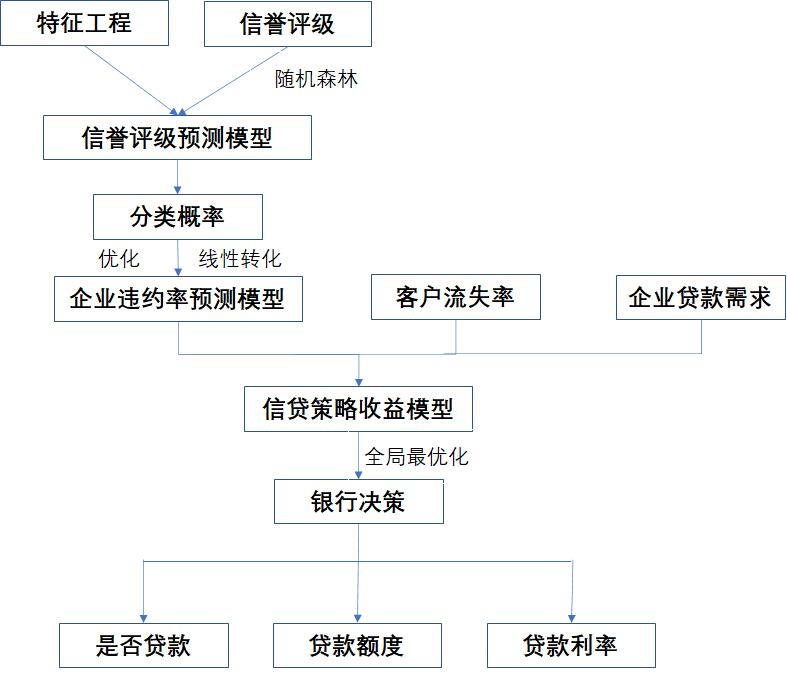
\includegraphics[width=0.8\linewidth]{figures/figure1.jpg}  %插入的图,包括JPG,PNG,PDF,EPS等,放在源文件目录下
	\caption{模型思路框示意图}  %图片的名称
	\label{fig:mcmthesis-logo}   %标签,用作引用
\end{figure}

\newpage

\section{\heiti 特征工程}
\subsection{\heiti 新特征构建及原因分析}
  \indent 根据问题分析中所述,我们根据财务指标与非财务指标类下的九项指标,分别构建一定程度能反映该指标的新特征,构建特征与构建原因见下表:

\begin{figure}[h]%%图
	\centering  %插入的图片居中表示
	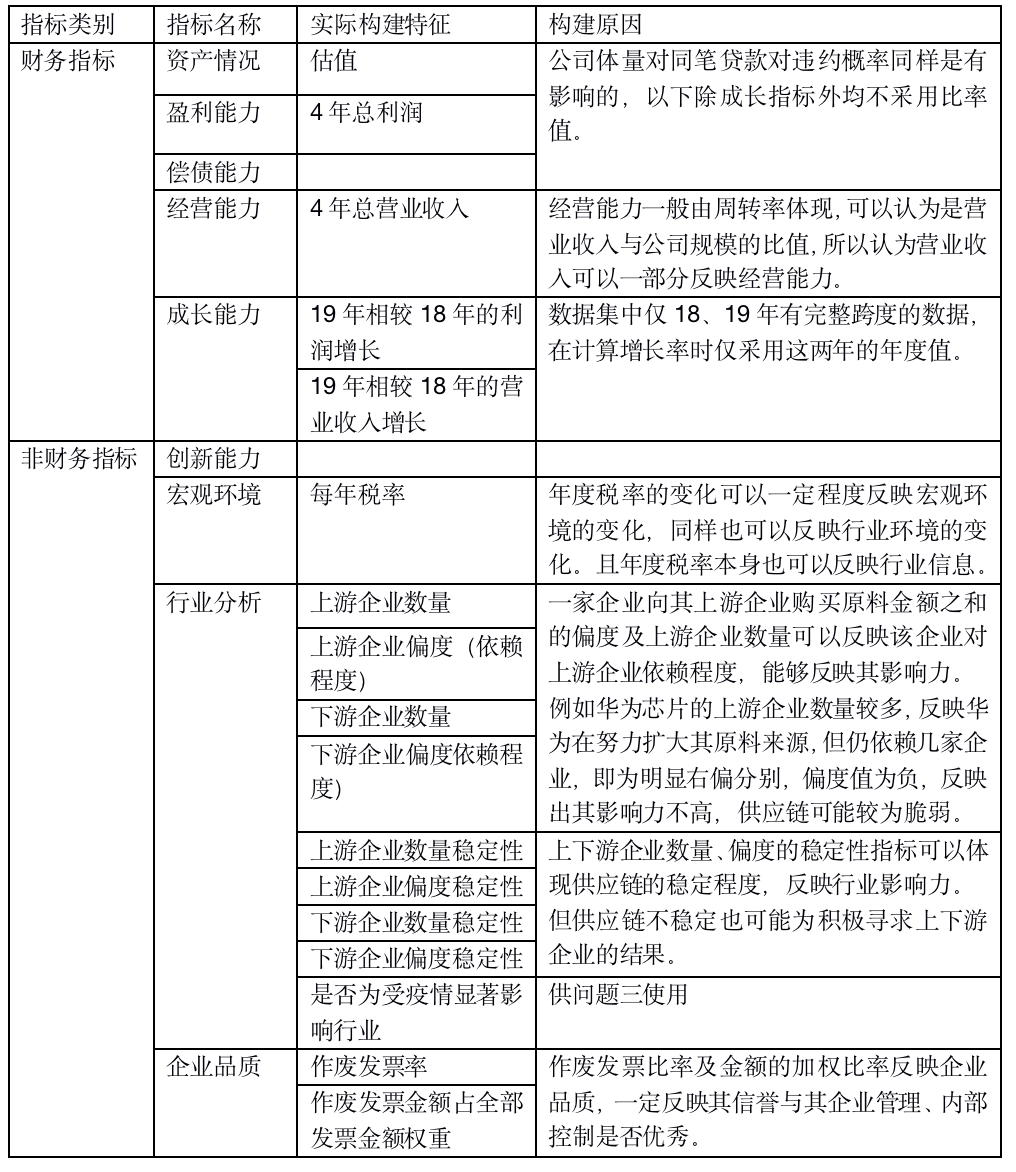
\includegraphics[width=1\linewidth]{figures/figure2.jpg}  %插入的图,包括JPG,PNG,PDF,EPS等,放在源文件目录下
	\label{fig:mcmthesis-logo}   %标签,用作引用
\end{figure}

\newpage
\subsection{\heiti 新特征构建方法及所用假定}

\noindent 由于数据受限,在构建特征时结合中小微企业特点作出以下假定:\\
 1、假定中小微企业无投资与筹资活动 ,现金流均为经营现金流。\\
2、假定流出经营现金流仅有税额与成本,均被发票信息记录。\\
\indent 2.1 假定中小微企业的人工成本不以工资的现金流流出体现。\\
\indent 2.2 假定不考虑其余经营活动的现金流出。\\
3、假定经营现金流入仅为出售商品所得的现金流入。\\
由2,进项发票 “价税合计” 之和 为流出经营现金流,即成本。\\
由3,销项发票 “价税合计” 之和 为流入经营现金流,即营业收入。\\

\noindent 自由现金流估值模型如下:\\
$Value = \sum_{t = 1}^{T} \frac{FCF_t}{(1+R_m)^t} +FCF_{T+1}*\frac{1}{R_m-g}*\frac{1}{(1+R_m)^T} $\\
其中Value为当前估值;\\
$FCF_t$为当前往后第t年的自由现金流预测值,预测中采用18与19年完整数据,预测其按该比率增长;\\
$R_m$为市场回报,取2019年沪深三百回报率36.07\%;\\
$g$表示T年后,假定自由现金流均以$g$同比例增长,假定g为10\%.
\begin{figure}[h]%%图	
	\centering  %插入的图片居中表示
	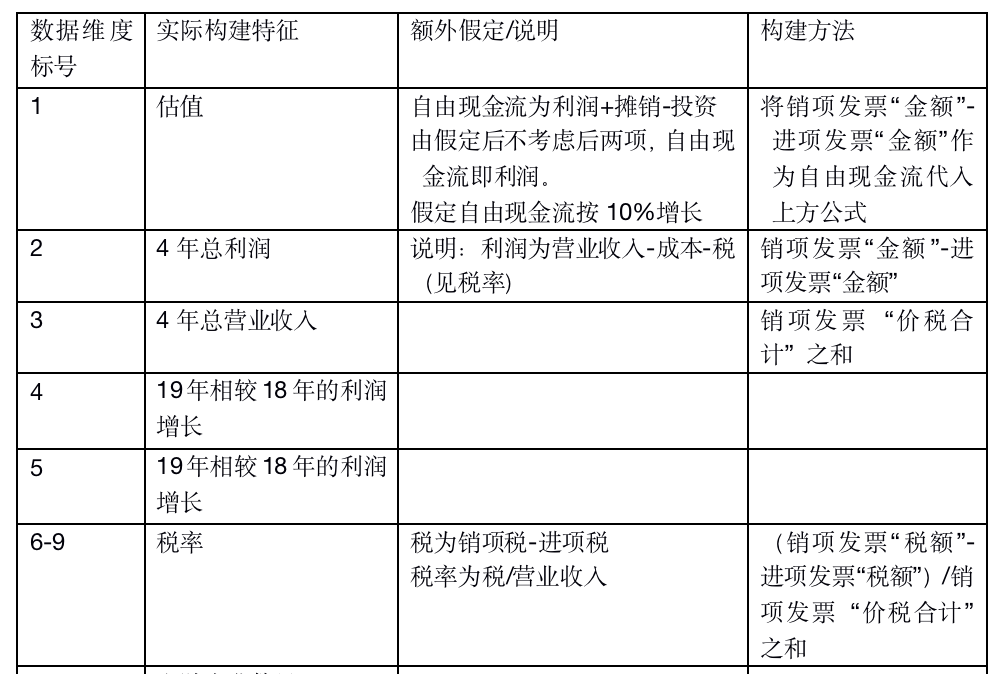
\includegraphics[width=1\linewidth]{figures/figure3.jpg}  %插入的图,包括JPG,PNG,PDF,EPS等,放在源文件目录下
	\label{fig:mcmthesis-logo}   %标签,用作引用
\end{figure}
\newpage
(接上图)\\
\begin{figure}[h]%%图	
	\centering  %插入的图片居中表示
	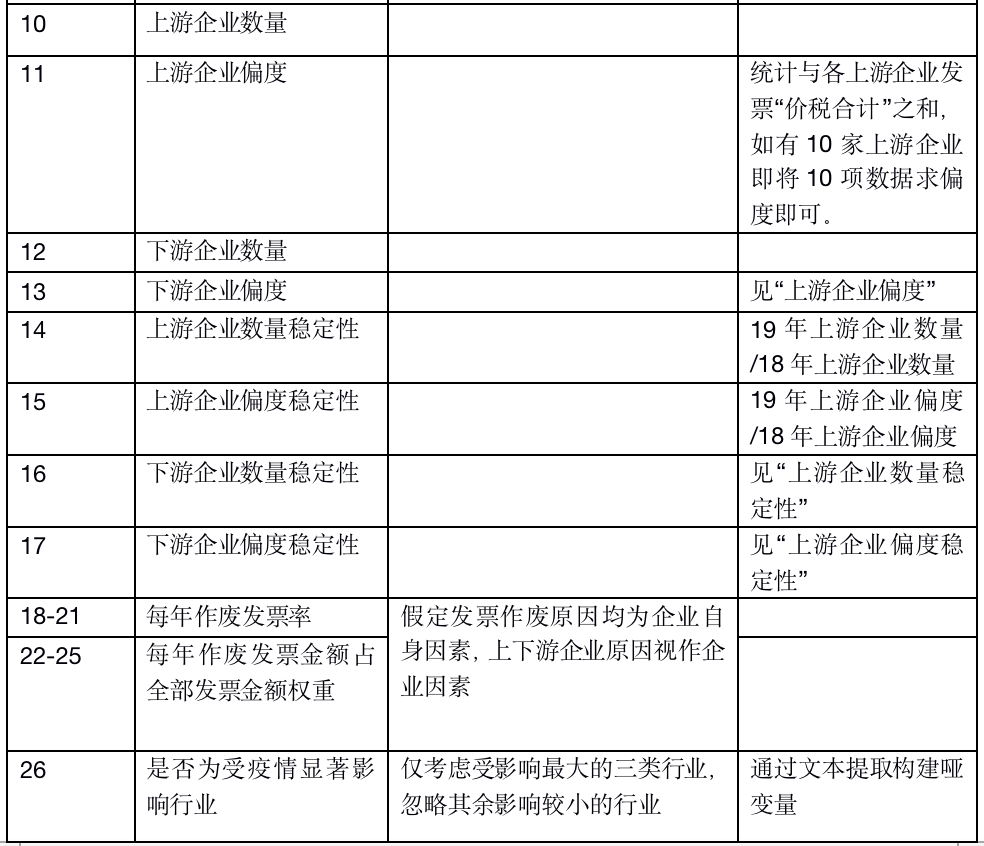
\includegraphics[width=1\linewidth]{figures/figure4.jpg}  %插入的图,包括JPG,PNG,PDF,EPS等,放在源文件目录下
	\label{fig:mcmthesis-logo}   %标签,用作引用
\end{figure}
%%%%%%%%%%%%%%%%%%%%%%%%%%\begin{itemize}[itemindent=1em]
%\item 假设题中所给的数据获取方式和来源具有可靠性和真实性且对模型稳定性无影响。\par
%%\item 假设题中一月部分数据(与二三四月数据波动趋势明显不符)对整体模型的构建影响不大。\par
%%\item 假设题中所有原始数据具有实时性。\par
%%%%%%%%%%%%%%%%%%%%%%%%%%\end{itemize}

\newpage
\section{\heiti 符号说明}
\begin{tabular}{cc}
	\hline
	\makebox[0.4\textwidth][c]{符号及名词}	&  \makebox[0.5\textwidth][c]{意义} \\ \hline
	$i$	    & 第i家企业\\ \hline
	$(p_1,p_2,p_3,p_4)_i$	    & 第i家企业“信誉评级”为A、B、C、D的概率\\ \hline
	$(\lambda_1,\lambda_2,\lambda_3,\lambda_4)$ & A、B、C、D“信誉评级”对应的违约概率  \\ \hline
	$k_i$	    & 是否给第i家企业贷款  \\ \hline

	$x_i $    & 给第i家企业贷款金额 \\ \hline
	$r_i $	    &  给第i家企业贷款利率 \\ \hline
	$a_i $	    & 第i家企业流失概率  \\ \hline
	$b_i$         & 第i家企业违约概率  \\ \hline
	$E_i$         & 第i家企业的贷款收益  \\ \hline
	$f_i$         & 第i家企业的贷款需求  \\ \hline
	$\bold{X} $	    & 所有企业的贷款金额 (向量) \\ \hline
	$\bold{R} $         & 所有企业的贷款利率(向量) \\ \hline
	$E$         & 总贷款收益  \\ \hline
	$S$         & 年度信贷总额  \\ \hline
	
	
	\hline
\end{tabular}



\begin{center}
\end{center}




\newpage

\section{\heiti  模型建立与求解}



\subsection{\heiti 问题一、二模型的建立与求解}
\noindent \textbf{ 5.1.1最优化问题建立}\\
\indent 根据问题分析“2.1.1 最优化策略”的描述,考虑到: 1、对于中小微企业的信贷策略,银行放贷对象较多且金额较为分散,使得一定程
度上已经实现了风险的分散化。 2、中小微企业的信贷策略可以具有一定风险偏好,将贷款放给有一定风险但能接
受更高利息的企业,该类企业往往是更为需要贷款资金的,且我们也能得到更高回报。所以我们基础限定违约率(风险)最大值,寻求利润期望的最大化策略。
\\\indent 又根据问题分析“2.1.5 贷款需求”的描述,考虑到:1、“贷款需求”实际与“贷款利率”的影响类似,公司考虑自身发展考虑,对不同额
度贷款的接受概率应当不同,但并无该类数据。2、
通过自由 现金流模型对企业估值来预测其贷款需求额度,并由于额度仅 10-100 万跨度不大,所 以我们可以作出假定,基于估值合理预测了贷款需求后,公司的接受概率无该额度大小 无关,仅与利率相关。
\\\indent 所以我们在基于合理评估贷款额度与限定违约率(风险)最大值的前提下,寻求利润期望的最大化策略,数学语言如下:
\begin{displaymath}
\bold{x}^*, \bold{y}^*,\bold{k}^* =\arg_{\bold{x}, \bold{y},\bold{k} }\max E \\
\end{displaymath}
subject to
$$ E_i =k_i[x_i y_i (1-a_i)(1-bi)-x_i(1-a_i)b_i]$$
$$ E=\sum_i E_i$$
$$x_i \in [10w, 100w]$$
$$\sum_i x_i k_i\leq S$$
$$k_i\in\{0,1\}$$
$$y_i \in [4\%,15\%]$$
$$x_i\in [80\% f(x_i),120\% f(x_i)]$$\\
\indent 投资策略的利润的期望为放贷给 各企业利润的期望的和,而对于单个利
润的期望值取决于是否放贷、放贷额度多少、贷款利率多少,以及企业接受该利率贷款 的概率、违约的概率等因素。其中是否放贷、放贷额度多少、贷款利率多少是我们投资 策略的具体决策,即我们针对上述带约束的最优化问题进行后续建模求解的目标。而企 业接受该利率贷款的概率可从客户流失率估计,我们仍需要估计出企业违约的概率。\\
\indent 由于题目中并未给出“违约概率”,针对问题一,我们从已有信息入手,分析发现有信贷记录的 123 家企业的企业信息中,“信誉评级”及“是否违约”两项指标与“违 约概率”相关。且观察可知,“是否违约”信息已被“信誉评级”信息涵盖,所以,“信 誉评级”能较好地反映企业的“违约概率”。我们只需要找到“信誉评级”与“违约概 率”合适的对应关系,即可以估计出企业的“违约概率”。\\
\indent 针对问题二,没有信贷记录的 302 家企业我们没有“信誉评级”数据,从而我们利
用问题一的“信誉评级”信息及其余数据构建的特征作为训练集来训练随机森林模型以
预测其“信誉评级”,从而由问题一的对应关系得到其“违约概率”。 并且,随机森林模型预测的各企业各“信誉评级”的概率值比直接给出其“信誉评级”
涵盖更多信息。因此问题一、二中均可采用随机森林预测的企业各“信誉评级”的概率 值与“违约概率”的对应关系代替原“信誉评级”与“违约概率”关系以计算“违约概率”。



\noindent \textbf{ 5.1.2信誉评级分类概率预测}\\
\indent 首先,根据分析的“2.1.6预测模型”中所述思路,我们将123组由信贷记录中小微企业经特征工程处理完后的25维数据(暂不考虑特定行业特征)与“信誉评级”作为训练集,将无信贷信息的302家中小微企业按相同处理作为测试集,代入随机森林模型。\\
模型的输入输出如下:(N 为中小微企业数量)\\
N*25的输入矩阵:将原有数据按上述特征处理后的25维数据。\\
N*4的输出矩阵为:各中小微企业“信誉评级”分别为A、B、C、D的概率值.\\
\\
 ( 在预测过程中,我们尝试使用了朴素贝叶斯、神经网络、支持向量机、随机森林、逻辑回归等不同算法。逻辑回归与朴素贝叶斯方法的准确率较低(约为70\%),神经网络的运行时间过长,支持向量机算法并不支持计算获得其他评级的概率,我们最终选择了随机森林算法(通过搭建多颗决策树并将它们合并,最终得到更稳定且准确的结果)。)\\
\\
\noindent \textbf{ 5.1.2.1 问题一分类概率结果}\\
\indent 有信贷记录的123家企业的“信誉评级”分别为A、B、C、D的概率值见\textbf{"附录1"},以下举代号为E1、E50、E100的企业的结果做说明:\\
\indent E1企业“信誉评级”分别为A、B、C、D的概率值为(0.82,0.11,0.06,0.01),即E1有82\%的概率“信誉评级”为A,11\%的概率“信誉评级”为B,6\%的概率“信誉评级”为C,1\%的概率“信誉评级”为D,而E1原数据中给出评级为A,说明较为判断合理。\\
\indent E50企业“信誉评级”分别为A、B、C、D的概率值为(0.01,0.29,0.69,0.01),E50原数据中给出评级为C,说明较为判断合理。\\
\indent E100企业“信誉评级”分别为A、B、C、D的概率值为(0.03,0.05,0.17,0.75),E50原数据中给出评级为D,说明较为判断合理。\\

\noindent \textbf{ 5.1.2.2 问题二 分类概率结果}\\
\indent 无信贷记录的302家企业的“信誉评级”分别为A、B、C、D的概率值见\textbf{"附录2"},以下举代号为E1、E50、E100的企业的结果做说明:\\
\indent E1企业“信誉评级”分别为A、B、C、D的概率值为(0.33,0.44,0.15,0.06),即E1有33\%的概率“信誉评级”为A,44\%的概率“信誉评级”为B,15\%的概率“信誉评级”为C,6\%的概率“信誉评级”为D,我们预测其信誉评级为B。\\
\indent E100企业“信誉评级”分别为A、B、C、D的概率值为(0.17,0.36,0.3,0.17),我们预测其信誉评级为B。\\
\indent E200企业“信誉评级”分别为A、B、C、D的概率值为(0.03,0.05,0.17,0.75),我们预测其信誉评级为D。\\

\noindent \textbf{ 5.1.2.3 问题二“信誉评级”预测结果}\\
\indent 无信贷记录的 302 家企业的“信誉评级”预测\textbf{"附录3"},其中预测评级为B的企业数最多,符合一般认知。\\
\\
\noindent \textbf{ 5.1.2对应关系}\\
\indent  同样根据问题分析“2.1.6预测模型”中所述思路,“信誉评级”分别为A、B、C、D的分类概率并不能直接用于我们投资策略的决策选择,我们需要寻找合适对应关系,将“信誉评级”的分类概率线性转换为该企业的违约概率。即找到合适的A、B、C、D的分类概率对应的违约率百分数($\lambda_1,\lambda_2,\lambda_3,\lambda_4$),令$b_i = \lambda_1 p_1 +  \lambda_2 p_2 + \lambda_3 p_3 + \lambda_4p_4$。

\indent  根据“中国人民银行副行长陈雨露24日在国新办发布会上表示,2019年,我国商业银行的平均不良贷款率只有1.86\%,中小企业不良贷款率略微高于平均水平,但也远低于5\%的监管标准。”且由预测评级为 B 的企业数最多,我们尝试控制其在5\%以下,并设定两个评估指标:\\
一为数值的评估指标:$score1 = (\sum \frac{b_i-\lambda}{100})/   123$\\
二为尺度的评估指标:$score1 = (\sum \frac{b_i-\lambda}{ (\lambda_4-\lambda_1)})/   123$

评估如下表:

 \begin{figure}[h]%%图	
	\centering  %插入的图片居中表示
	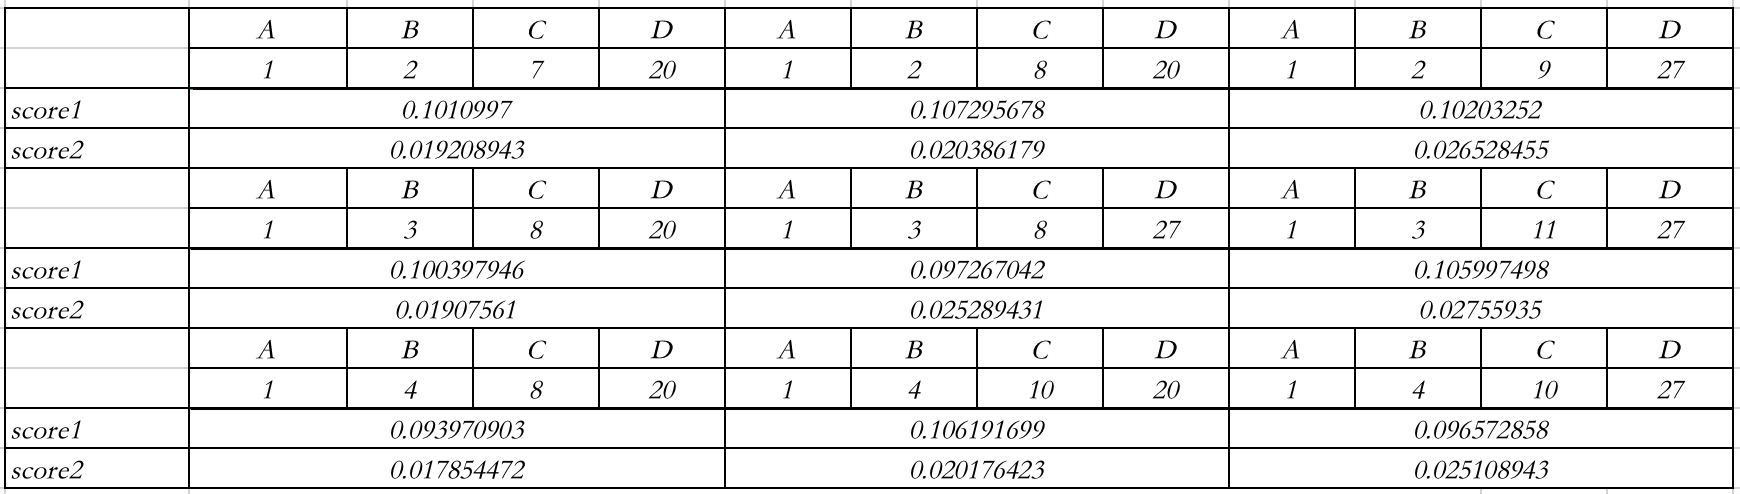
\includegraphics[width=0.8\linewidth]{figures/figure10.jpg}  %插入的图,包括JPG,PNG,PDF,EPS等,放在源文件目录下
	\label{fig:mcmthesis-logo}   %标签,用作引用
\end{figure}
由上表知“信誉评级”为A、B、C、D对应的违约概率百分数为1\%,3\%,9\%,27\%两项指标均较佳,因而我们采用该对应关系将“信誉评级”的分类概率的预测值转换为“违约概率”的预测值。\\
\\
\noindent \textbf{ 5.1.3 流失率估算}\\
\indent 我们通过分析 银行贷款年利率与客户流失率关系的2019年统计数据,将数据拟合成函数,来减小随机误差。其中,我们尝试用三次多项式、二次多项式进行拟合,三次函数有着更好的拟合效果(R值更高),而二次函数的R值与三次函数较为接近,由奥卡姆剃刀定律,即“简单有效原理”,我们采用二次多项式拟合结果来估算客户流失率$a_i$。得出以下结论:\\
对于信誉评级为A的客户,流失率$a_i=-76.41y_i^2+21.984y_i-0.6971$\\
对于信誉评级为B的客户,流失率$a_i=-67.933y_i^2+20.207y_i-0.6504$\\
对于信誉评级为C的客户,流失率$a_i=-63.942y_i^2+19.569y_i-0.6393$\\

 \begin{figure}[h]%%图	
	\centering  %插入的图片居中表示
	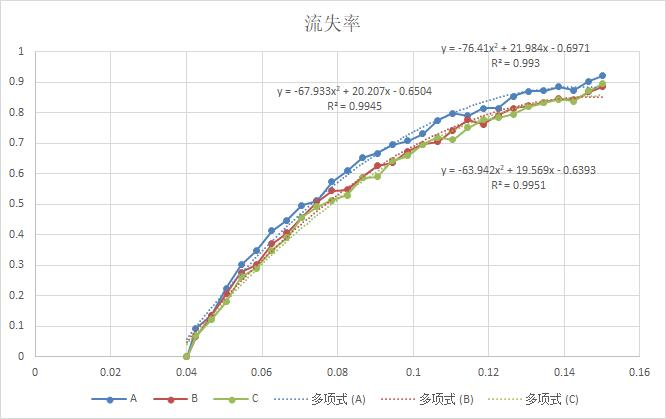
\includegraphics[width=1\linewidth]{figures/figure12.jpg}  %插入的图,包括JPG,PNG,PDF,EPS等,放在源文件目录下
	\label{fig:mcmthesis-logo}   %标签,用作引用
\end{figure}

 \begin{figure}[h]%%图	
	\centering  %插入的图片居中表示
	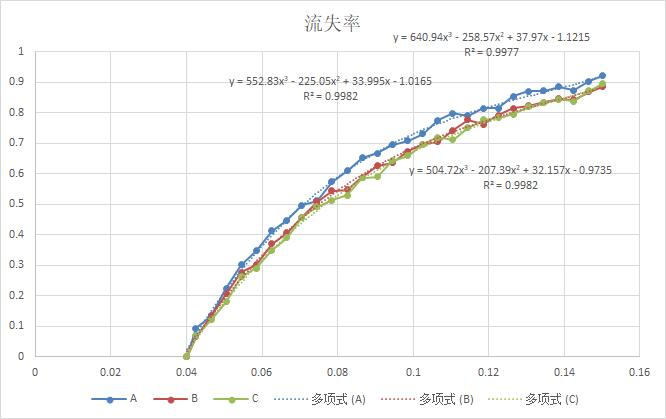
\includegraphics[width=1\linewidth]{figures/figure13.jpg}  %插入的图,包括JPG,PNG,PDF,EPS等,放在源文件目录下
	\label{fig:mcmthesis-logo}   %标签,用作引用
\end{figure}
\\
\newpage
\noindent \textbf{ 5.1.4 贷款需求额度预测}\\
由于没有直接给出各企业贷款需求额度的相关信息,我们通过预测企业估值,从而预测其贷款需求额度。\\
在去除一些估值为负数的公司后(同时,其信誉评级为D级),绝大多数公司的估值在100万至5000万。\\
我们预测,公司的贷款需求额度约为其估值的十分之一。而由于题目中银行贷款额度为10~100万元,我们对$f_i$进行定义。
\\

$$ 
f_i=\left\{
\begin{aligned}
 10^5 & (V_i\leq 10^6)\\
 \frac{V_i}{10} & (10^6<v_i<10^7)\\
 10^6 & (V_i\geq 10^7)\\
\end{aligned}
$$

\noindent \textbf{ 5.1.5 模型简化}\\
\indent 通过分析收益期望,我们发现:当且仅当$x_i y_i(1-b_i)(1-a_i)>x_i b_i (1-a_i)$时,银行放贷将获得收益。所以当$15\%>\frac{b_i}{1-b_i}$, 即当$b_i >13.04\%$时,银行应直接拒绝i企业的贷款。\\
由于数据量较大,我们无法直接通过优化原问题来得到最优解,于是,我们尝试引入启发式算法:\\
\indent 由公式可知,为了使期望利益最大化,我们需要最大化单位金钱所带来的收益。\\
\indent 我们先在不考虑年度信贷总额的情况下优化$E_i$,将$E_i/x_i$记作$z_i$,即表示对于i企业放贷,单位金钱给银行所带来的收益。\\
$z_i=y_i(1-b_i)(1-a_i)-b_i(1-a_i)$\\
\indent 将$z_i$由高到低排序,优先满足z更高的企业,直至放贷总金额达到年度信贷总额。\\
我们通过分析 银行贷款年利率与客户流失率关系的2019年统计数据,将数据拟合成函数,来减小随机误差。其中,我们尝试用三次多项式、二次多项式进行拟合,三次函数有着更好的拟合效果(R值更高),而二次函数的R值与三次函数较为接近,由奥卡姆剃刀定律,即“简单有效原理”,我们采用二次多项式拟合结果来估算客户流失率a_i。\\

$$z_i=y_i(1-b_i)(1-a_i)-b_i(1-a_i)$$
$$a_i=m_1y_i^2+m_2y_i+m_3$$
所以
$$z_i=y_i(1-b_i)(1-m_1 y_i^2-m_2y_i-m_3)-b_i(1-m_1y_i^2-m_2y_i-m_3)$$
为了得到z值的最优解,我们对其求导,使导数为零:
$$\frac{\partial z_i}{\partial y_i}=(1-b_i)(-2m_1y-m_2)y_i+(1-b_i)(1-m_1 y_i^2 -m_2y-m_3)+b_i(2m_1 y_i+m_2)$\\
$=(1-b_i)(-2m_1y_i^2-m_2y_i+1-m_1y_i^2-m_2y_i-m_3)+b_i(2m_1y_i+m_2) \\
=3(1-b_i)m_1y_i^2-2((1-b_i)m_2-b_im_1)y_i+b_i(m_2+m_3)+1-b_i$$
\\

\noindent \textbf{ 5.1.6 启发式算法}\\
\indent 由于数据量较大,我们无法直接通过优化原问题来得到最优解,于是,我们尝试引入启发式算法: \\
\indent 由公式可知,为了使期望利益最大化,我们需要最大化单位金钱所带来的收益。
我们先在不考虑年度信贷总额的情况下优化$E_i$,
将$E_i/x_i$ 记作$z_i$,$z_i=y_i(1-b_i)(1-a_i)-b_i(1-a_i)$,即表示对于i企业放贷,单位金钱给银行所带来的收益将$z_i$由高到低排序,优先满足z更高的企业,直至放贷总金额达到年度信贷总额。
\\

\noindent \textbf{ 5.1.7 结果反馈}\\
\noindent \textbf{ 5.1.7.1 对有信贷记录的123家企业的投资决策}\\
根据以上模型,我们得出了具体放贷决策,针对问题一,在信贷额度不确定情况下,按“附录5”所列企业顺序,按表中的金额($x_i$)、利率($y_i$)、是否放贷($k_i$)这一决策进行放贷,直至信贷额度用完。\\
\noindent \textbf{ 5.1.7.2 对无信贷记录的302家企业的的投资决策}\\
针对问题二,在信贷额度为1亿情况下,按“附录6”所列企业无次序放贷即可,对各企业决策为其代号行的金额($x_i$)、利率($y_i$)、是否放贷($k_i$)这一决策。


\subsection{\heiti 问题三模型的建立与求解}

不同行业来看,不同突发因素对于不同行业的企业有不同的影响,具体来说,我 们可以提高受影响行业对应特征的权重以放大其影响,由于问题二中模型各特征系数权重已确定,我们实际可以直接将行业特征的输入作放大处理,其等效于将行业特征的影响放大。通过查阅新闻数据,我们对各个企业的违约率做出调整,其中我们将住宿和餐饮企业的违约率乘以1.5、制造企业违约率乘以1.2,其余企业的违约率乘以1.1,作为在突发情况(新冠疫情)的影响下,企业预计的违约率。
即针对不同突发因素,我们将人为估计可能受突发因素影响的企业估计其违约率的放大系数,并通过先前的模型进行放贷策略的调整。\\
\indent 由我们模型可见,由于在数据中住宿和餐饮企业较少,所以整体放贷策略没有太大调整。而利率普遍增高0.1\%。在问题三的模型中,我们仅仅调整了违约率这单一影响因素,而在实际情况中,有如企业规模、上下游公司情况、政策等影响因素,需要进一步改进模型。\\

\noindent \textbf{  结果反馈}\\
针对问题三,在信贷额度为1亿情况下,按“附录7”所列企业无次序放贷即可,对各企业决策为其代号行的金额($x_i$)、利率($y_i$)、是否放贷($k_i$)这一决策。





\section{\heiti 模型优缺点}
\subsection{\heiti 模型优点}

模型优点:随机森林有着较高的准确率,同时在训练模型时花费的时间成本远小于神经网络等算法。在没有实际违约率参照的·情况下,我们通过线性转换,概率估计来预测违约率,能得到较为理想的结果
\\
在做全局最优化时,我们尝试引入启发式算法来化简运算过程,在实际情况中,我们将面临规模庞大的数据集,通过随机森林和启发式算法,我们能大大节约时间,算力成本\\


\subsection{\heiti 模型缺点}

 1、在信誉评级模型中,我们仅考虑了----,并未考虑行业地位等因素带来的影响\\企业违约率模型中,我们通过信誉评级线性转换得到违约率,但实际情况将更为复杂,线性模型较为简略\\由于没有真实的违约率做参考,我们所得到的违约率转换仅仅是通过查阅资料,总结得出,真实情况下还需调整。\\

2、信贷策略收益模型中,由于只是对于期望求解,在真实环境中可能存在一定偏差,同时也要考虑不同银行的风险偏好不同,需要做出一些调整。\\
企业贷款需求的预测是通过公司估值得出的,模型较为简单,实际环境中,还需考虑行业、体量等因素。\\
客户流失率是通过2019年的数据,用多项式函数拟合得出,存在一定的误差,同时还需考虑每年的经济形势对流失率的影响。\\


3、在问题三的模型中,我们仅仅调整了违约率这单一影响因素,而在实际情况中,有如企业规模、上下游公司情况、政策等影响因素,需要进一步改进模型。



\newpage

\begin{appendices}
 \noindent \textbf{附录一:有信贷记录的123家企业的“信誉评级”分别为A、B、C、D的概率值}
 \begin{figure}[h]%%图	
	\centering  %插入的图片居中表示
	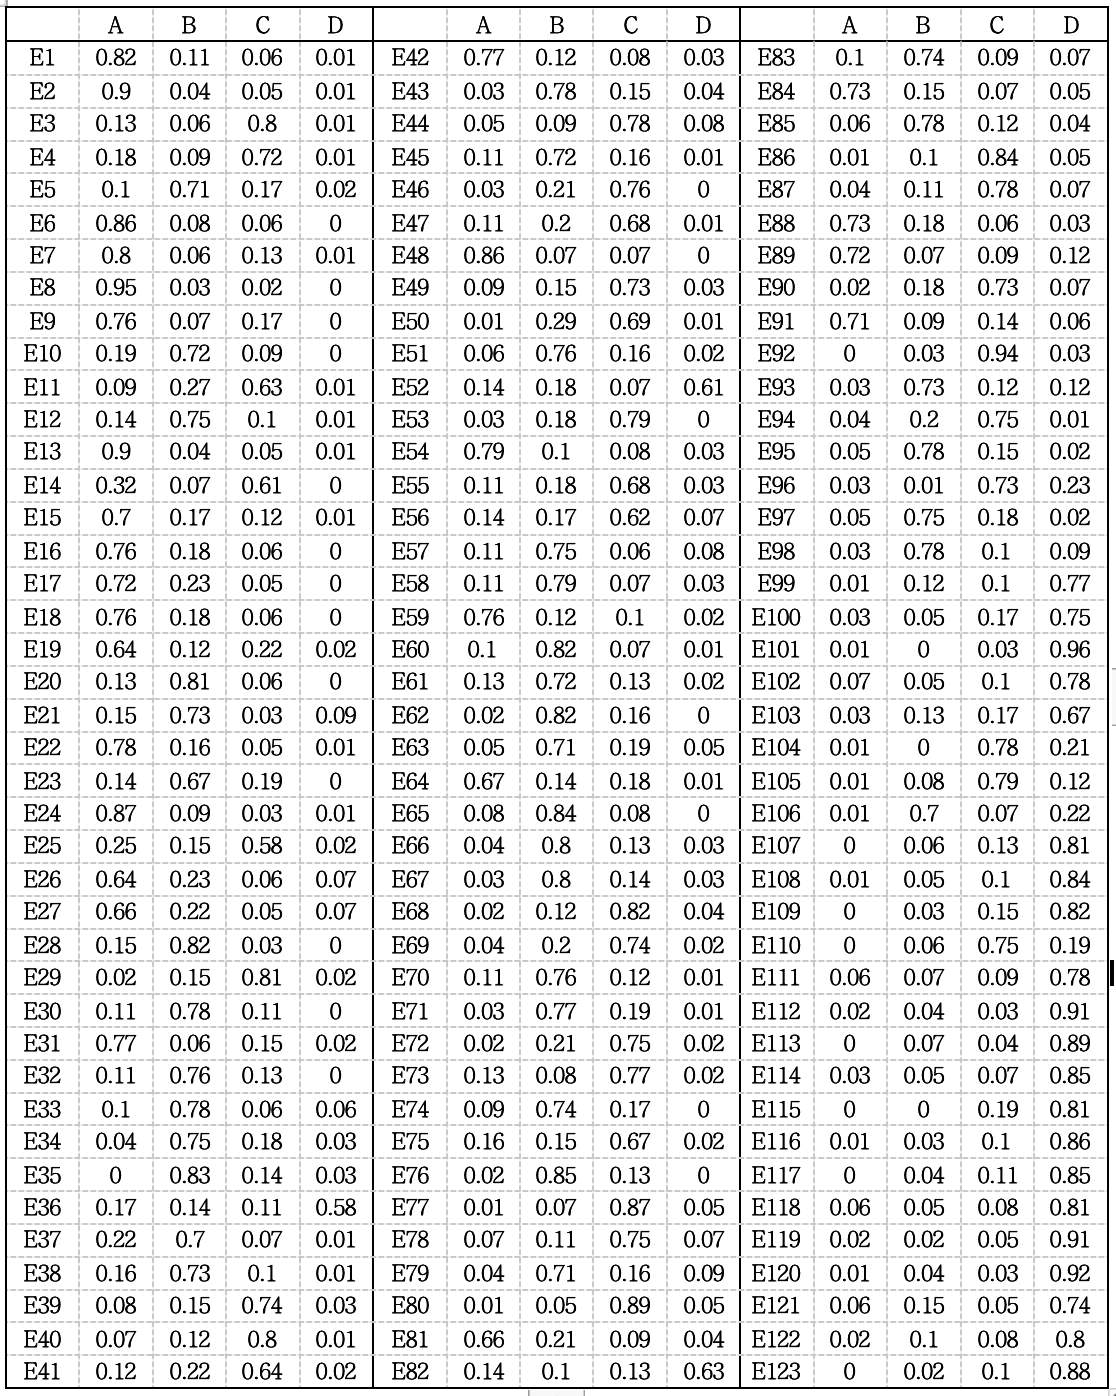
\includegraphics[width=1\linewidth]{figures/figure5.jpg}  %插入的图,包括JPG,PNG,PDF,EPS等,放在源文件目录下
	\label{fig:mcmthesis-logo}   %标签,用作引用
\end{figure}



\newpage
 \noindent \textbf{附录二:无信贷记录的302家企业的“信誉评级”分别为A、B、C、D的概率值(表中EN代表EN+123)}
 \begin{figure}[h]%%图	
	\centering  %插入的图片居中表示
	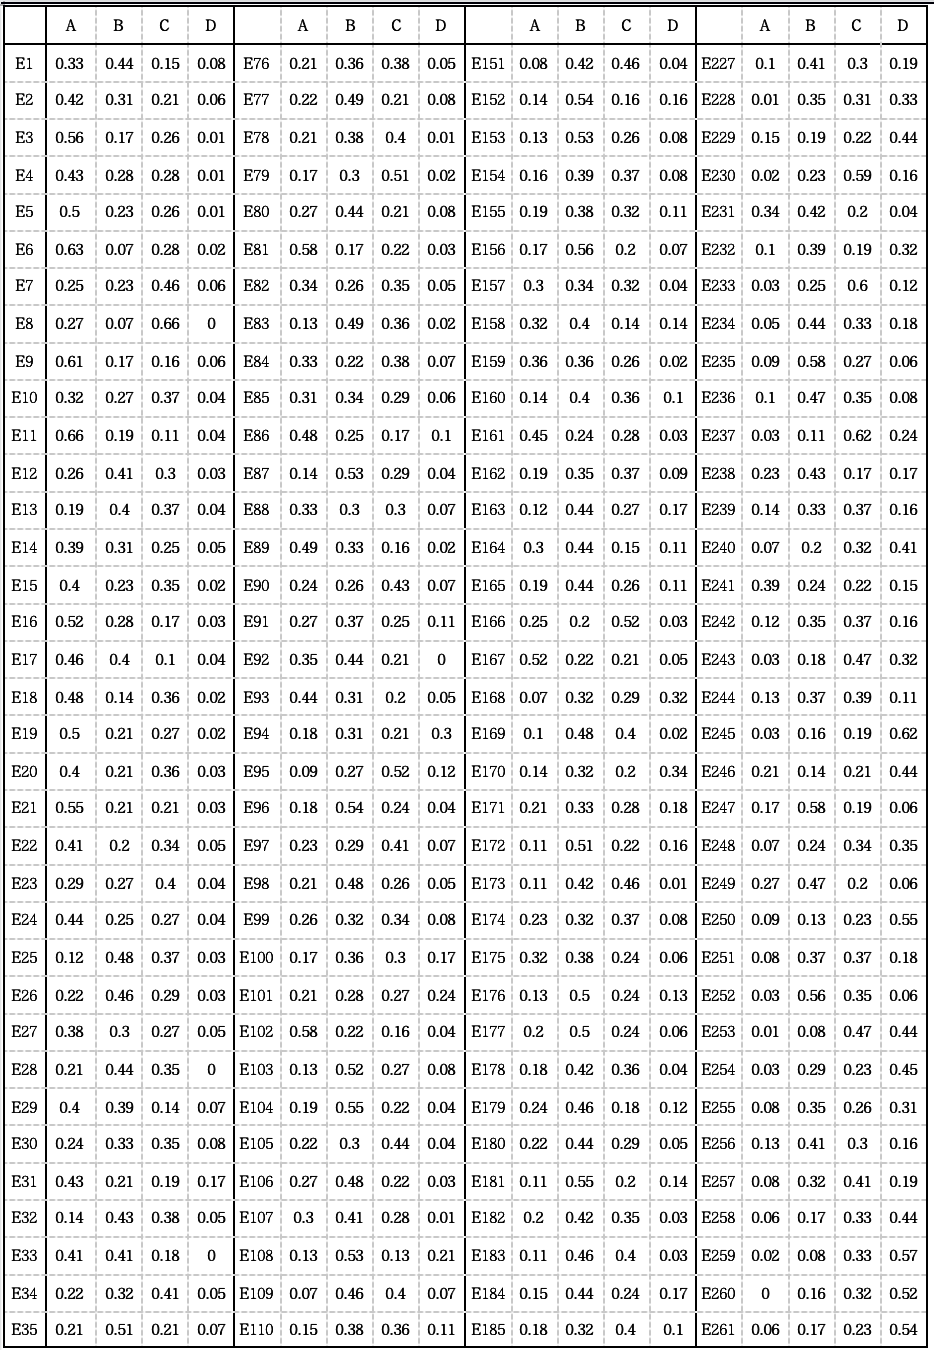
\includegraphics[width=0.95\linewidth]{figures/figure6.jpg}  %插入的图,包括JPG,PNG,PDF,EPS等,放在源文件目录下
	\label{fig:mcmthesis-logo}   %标签,用作引用
\end{figure}
\newpage
(接上表)(表中EN代表EN+123)
 \begin{figure}[h]%%图	
	\centering  %插入的图片居中表示
	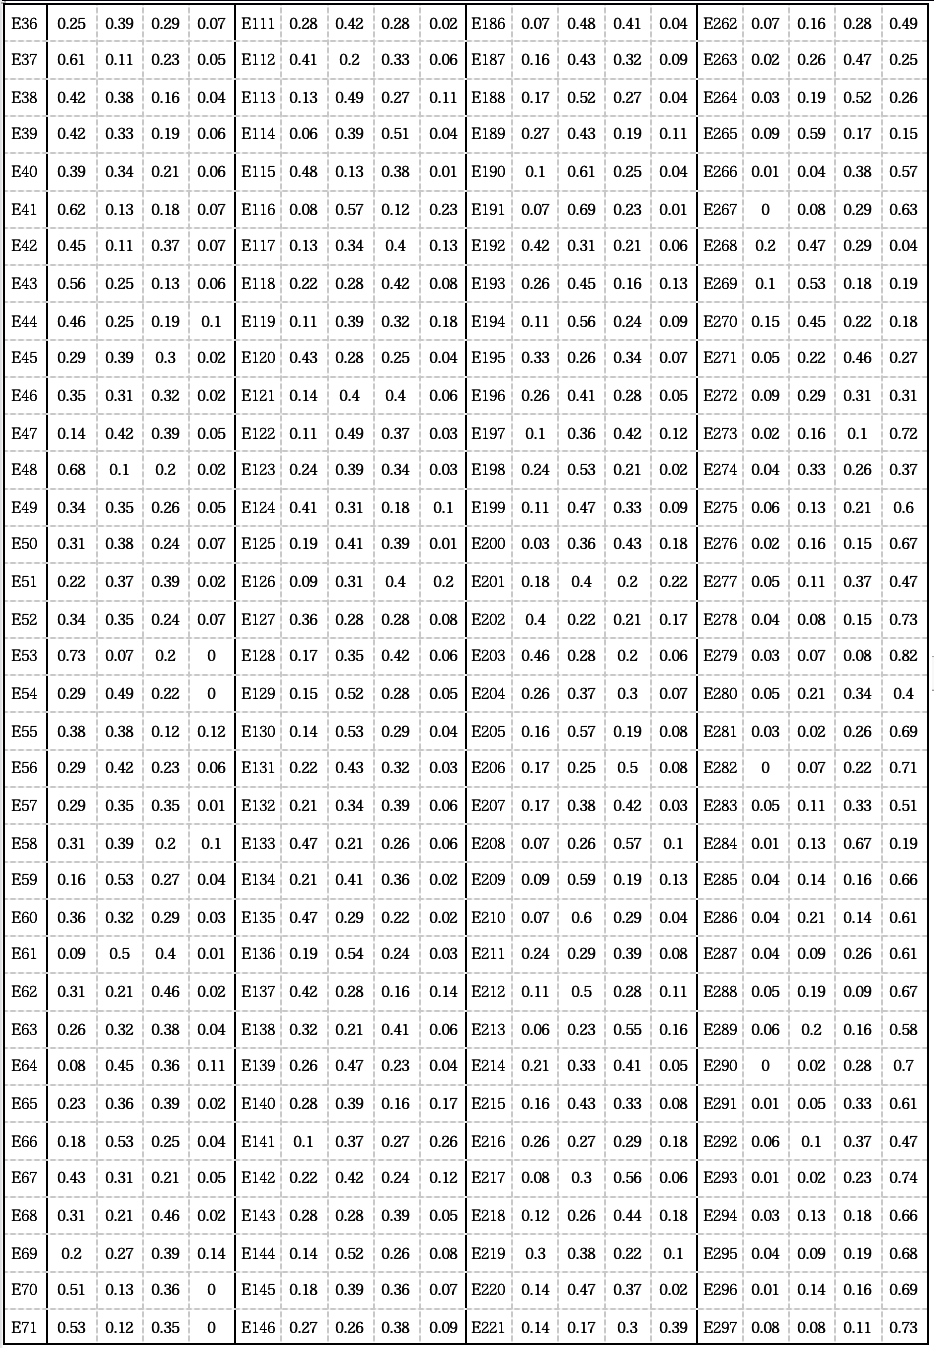
\includegraphics[width=0.95\linewidth]{figures/figure7.jpg}  %插入的图,包括JPG,PNG,PDF,EPS等,放在源文件目录下
	\label{fig:mcmthesis-logo}   %标签,用作引用
\end{figure}
\newpage

(接上表)(表中EN代表EN+123)
 \begin{figure}[h]%%图	
	\centering  %插入的图片居中表示
	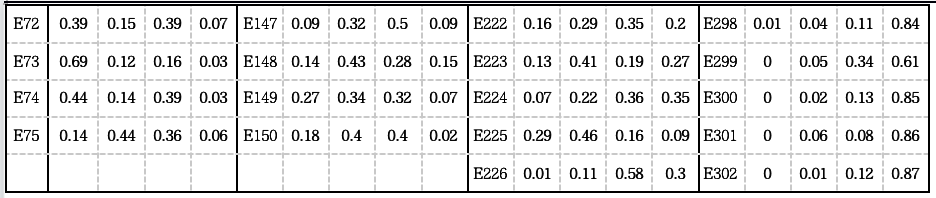
\includegraphics[width=0.95\linewidth]{figures/figure8.jpg}  %插入的图,包括JPG,PNG,PDF,EPS等,放在源文件目录下
	\label{fig:mcmthesis-logo}   %标签,用作引用
\end{figure}

\newpage
 \noindent \textbf{附录三:无信贷记录的302家企业的“信誉评级”预测}
 \begin{figure}[h]%%图	
	\centering  %插入的图片居中表示
	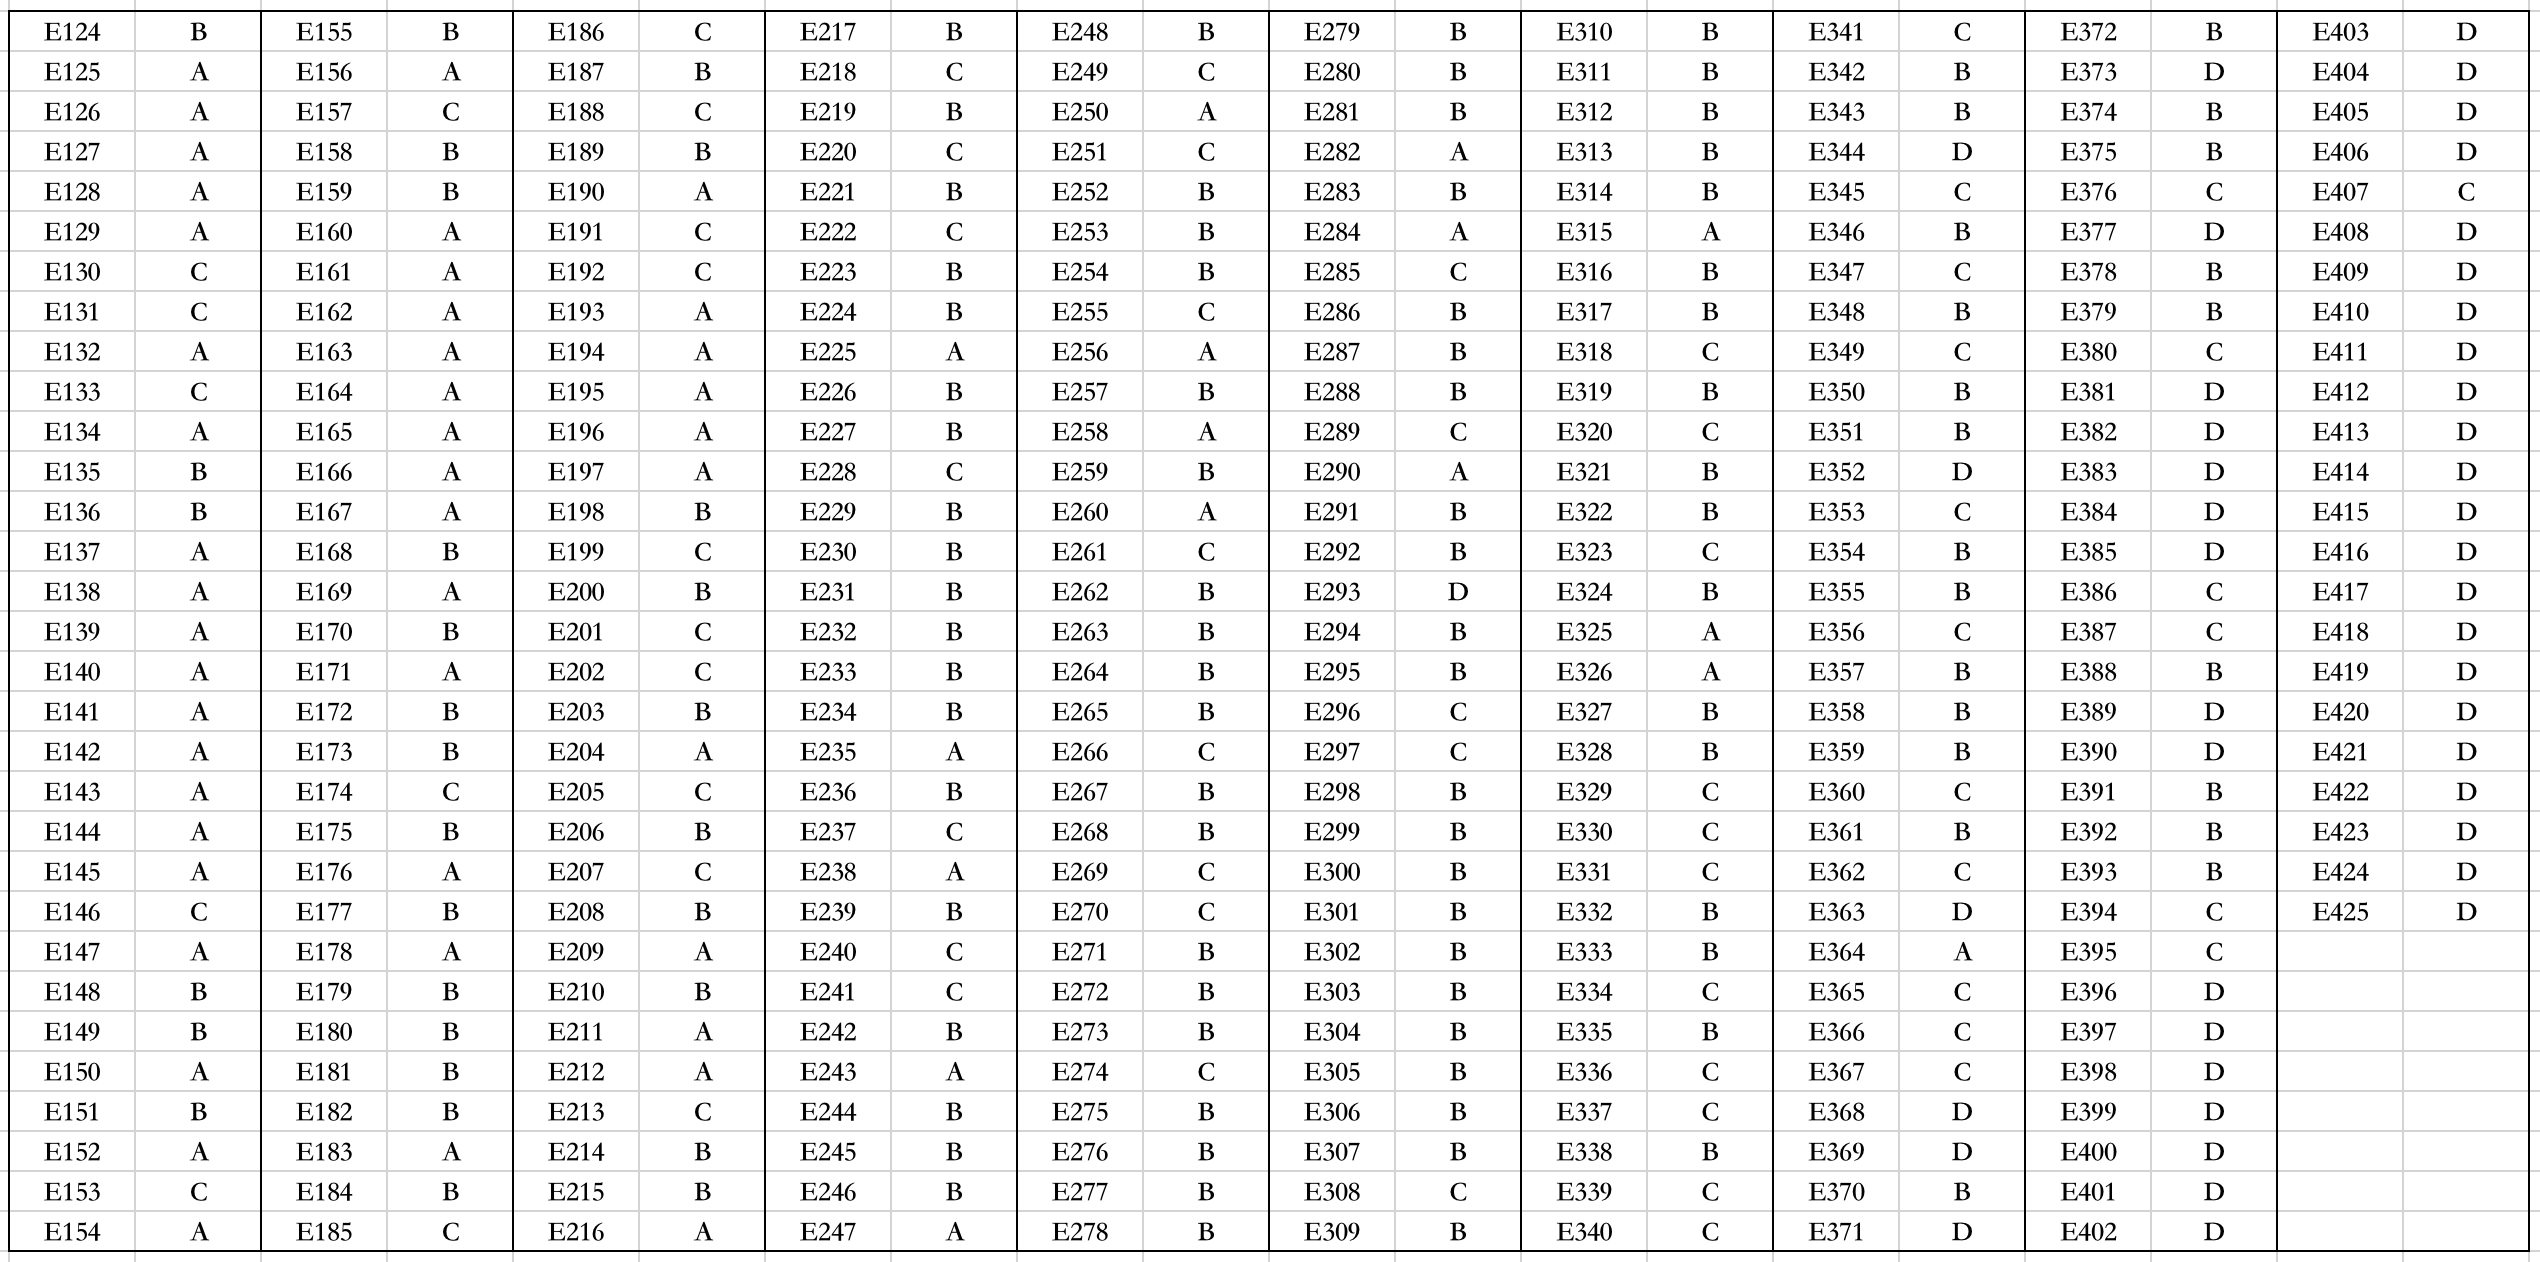
\includegraphics[width=1\linewidth]{figures/figure9.jpg}  %插入的图,包括JPG,PNG,PDF,EPS等,放在源文件目录下
	\label{fig:mcmthesis-logo}   %标签,用作引用
\end{figure}

\newpage
 \noindent \textbf{附录四:无信贷记录的302家企业的“信誉评级”预测}
 \begin{figure}[h]%%图	
	\centering  %插入的图片居中表示
	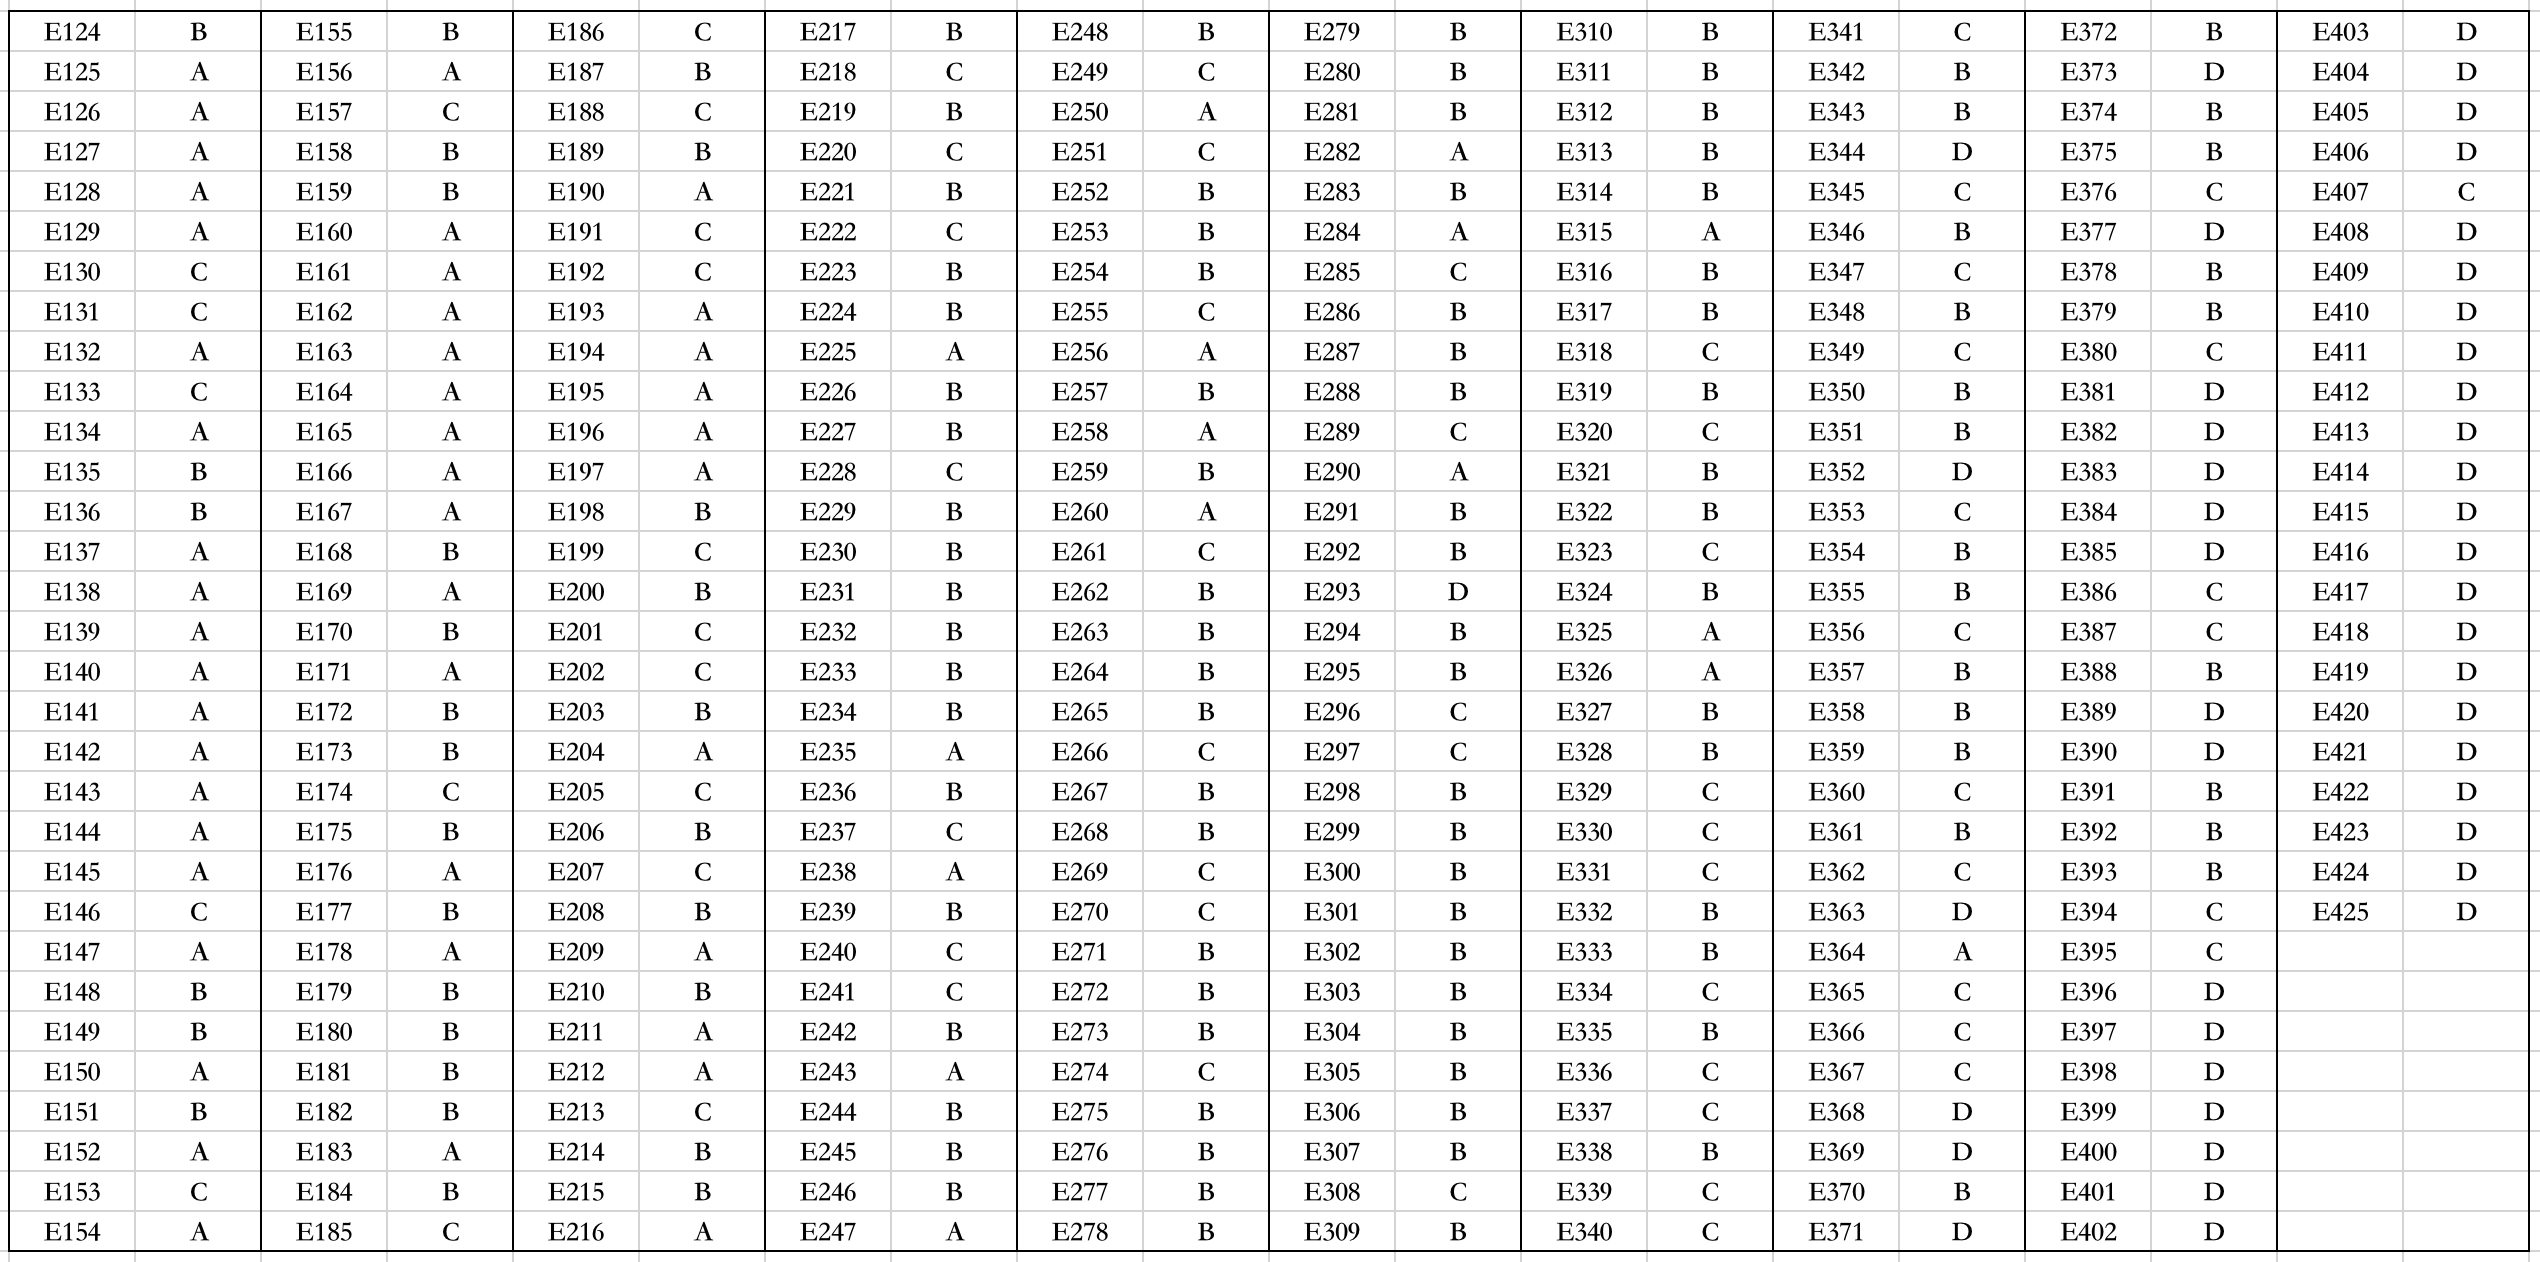
\includegraphics[width=1\linewidth]{figures/figure9.jpg}  %插入的图,包括JPG,PNG,PDF,EPS等,放在源文件目录下
	\label{fig:mcmthesis-logo}   %标签,用作引用
\end{figure}

\newpage
 \noindent \textbf{附录五:对有信贷记录的123家企业的投资决策}
 \begin{figure}[h]%%图	
	\centering  %插入的图片居中表示
	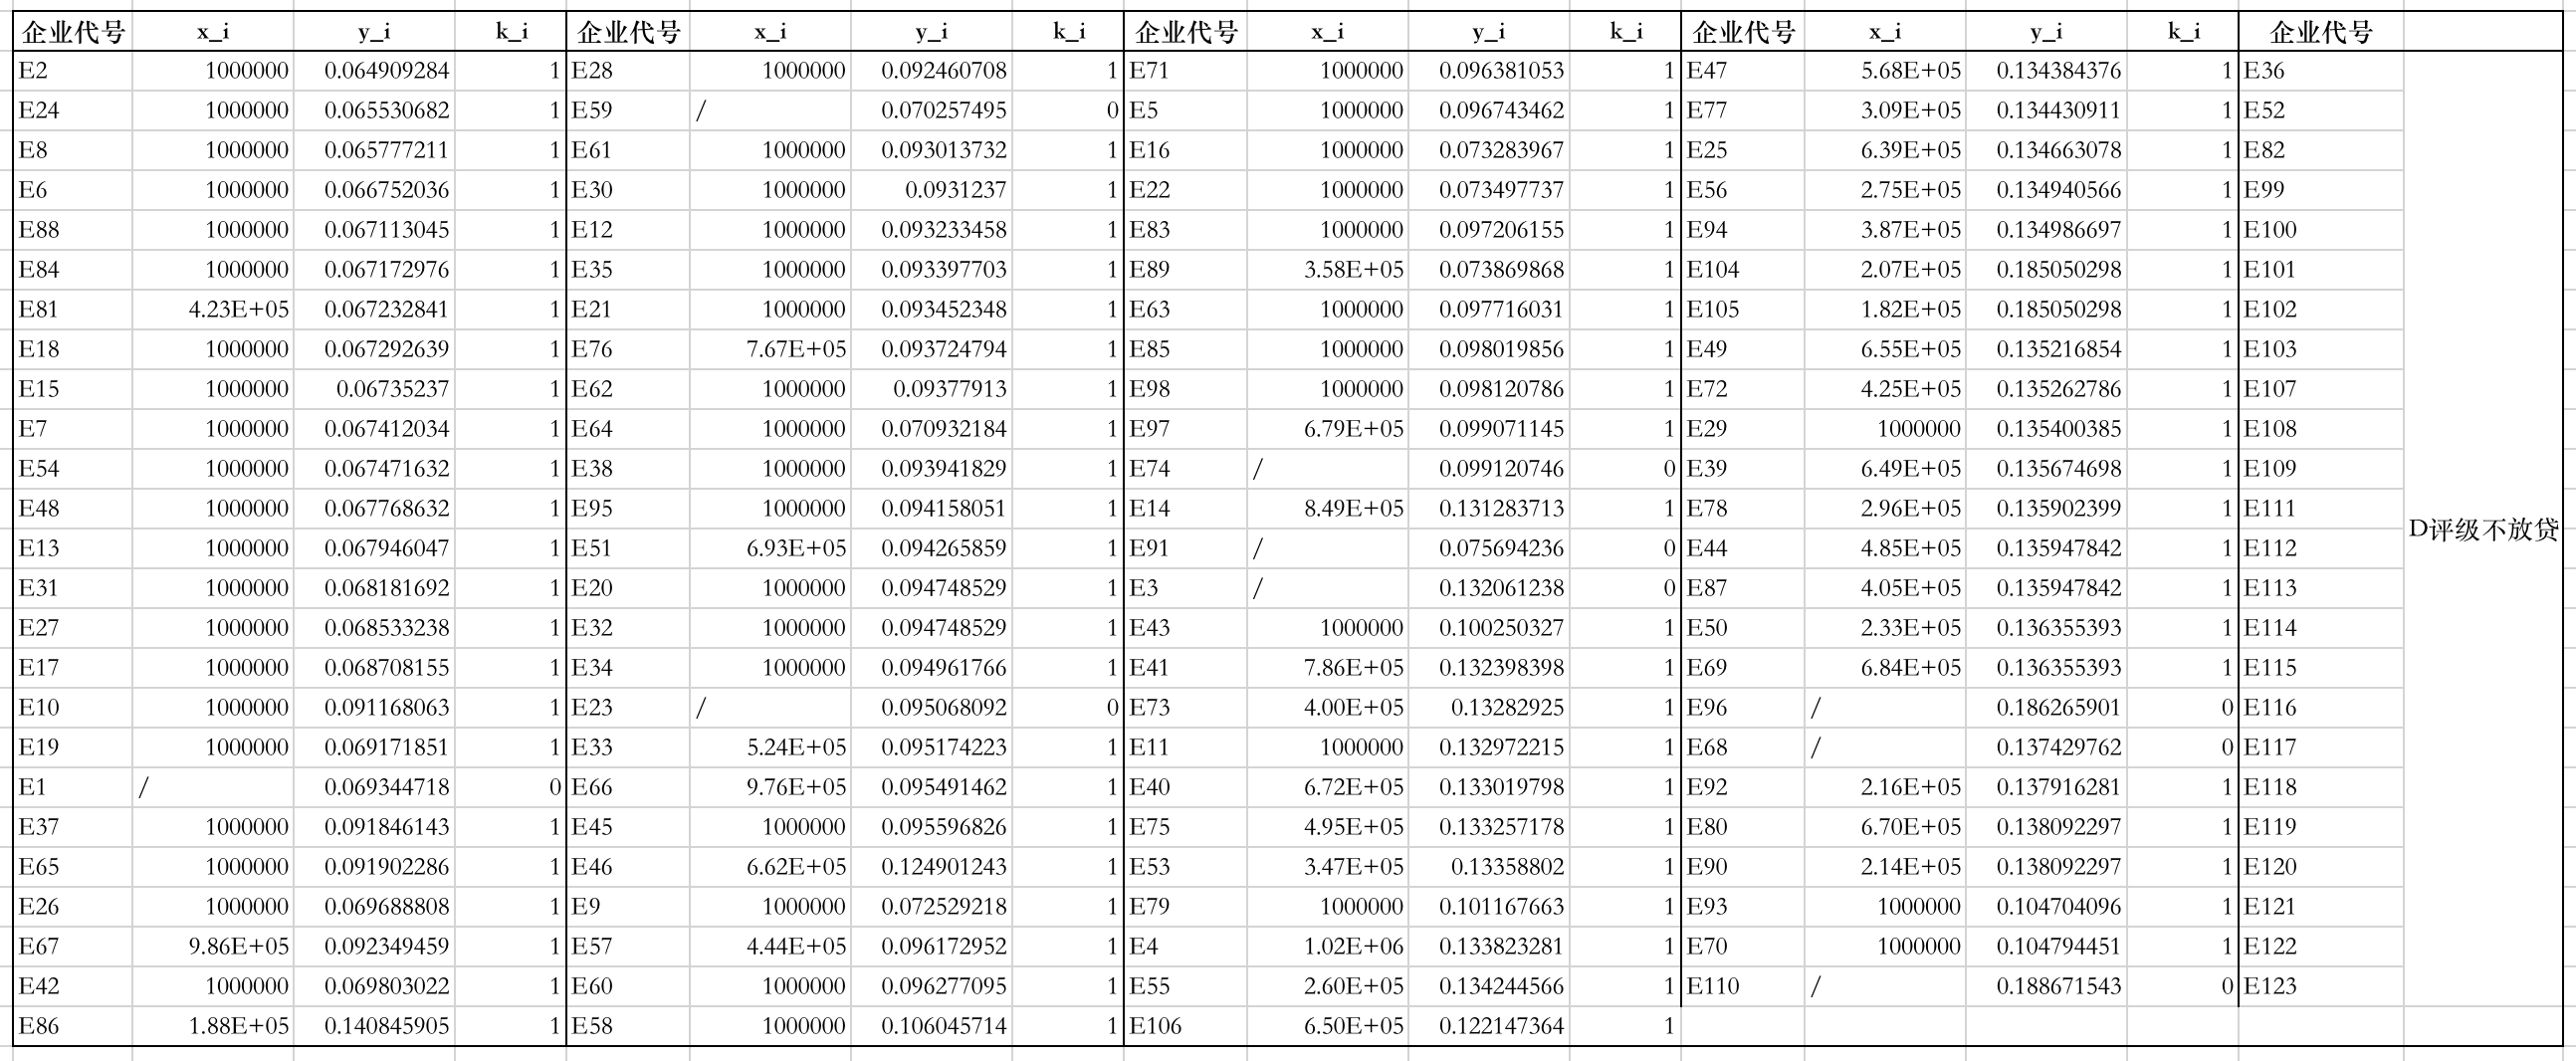
\includegraphics[width=1\linewidth]{figures/T1.jpg}  %插入的图,包括JPG,PNG,PDF,EPS等,放在源文件目录下
	\label{fig:mcmthesis-logo}   %标签,用作引用
\end{figure}

\newpage
 \noindent \textbf{附录六:对无信贷记录的302家企业的的投资决策}
 \begin{figure}[h]%%图	
	\centering  %插入的图片居中表示
	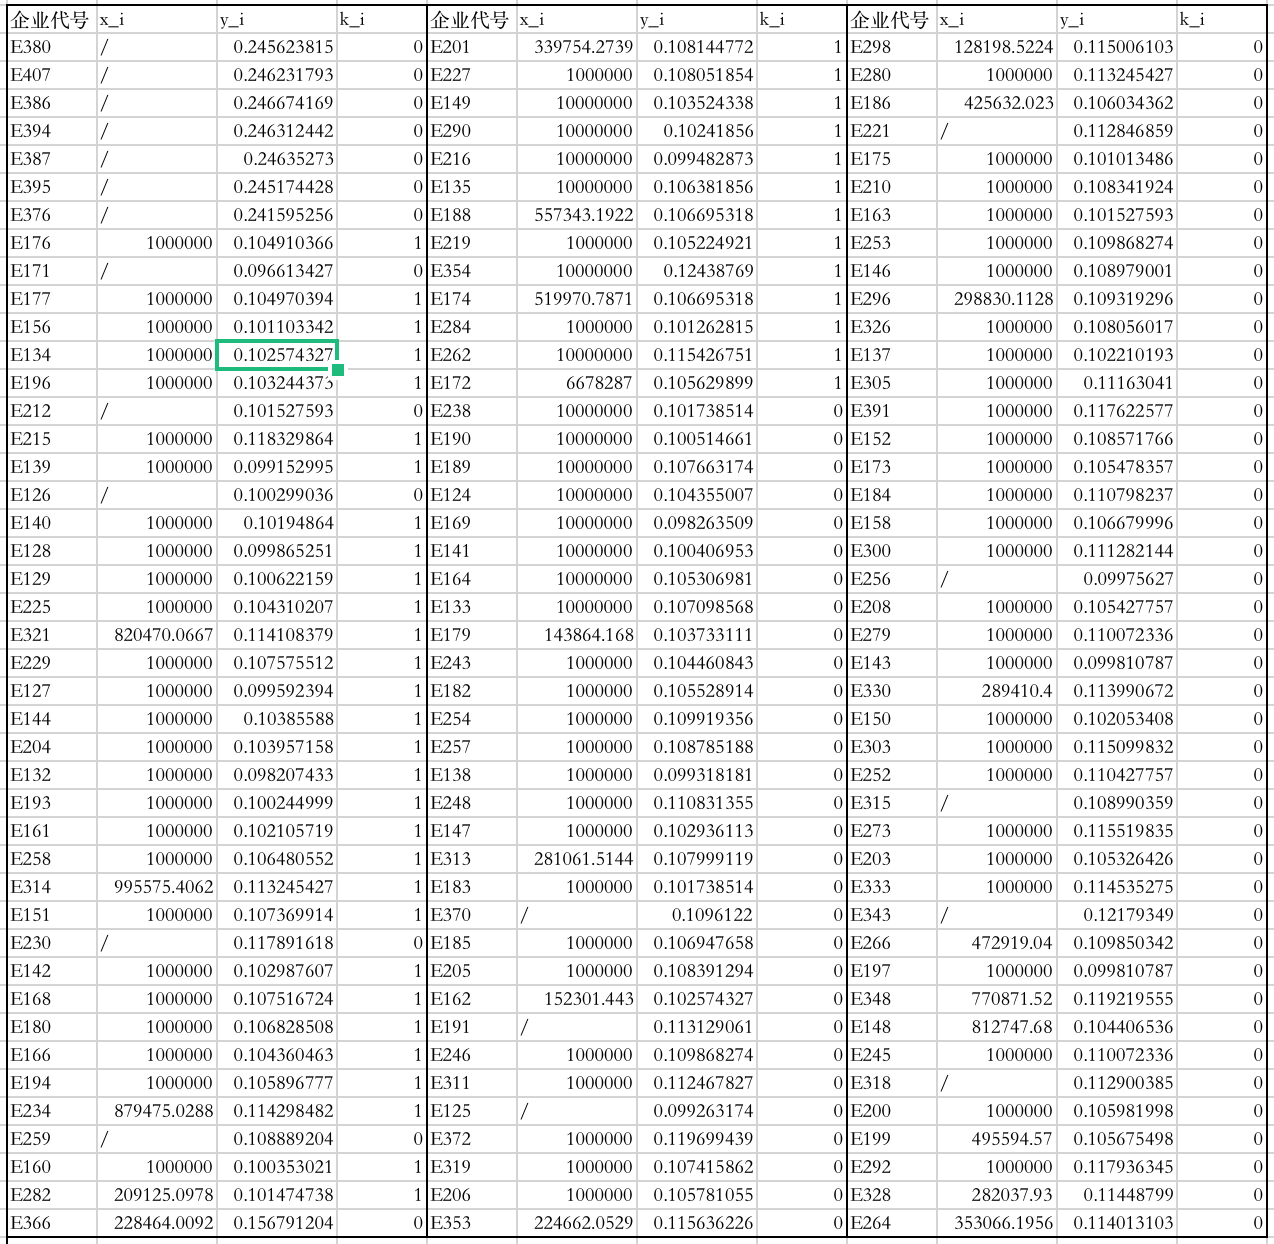
\includegraphics[width=1\linewidth]{figures/T2_1.jpg}  %插入的图,包括JPG,PNG,PDF,EPS等,放在源文件目录下
	\label{fig:mcmthesis-logo}   %标签,用作引用
\end{figure}

\newpage
(接上表)
 \begin{figure}[h]%%图	
	\centering  %插入的图片居中表示
	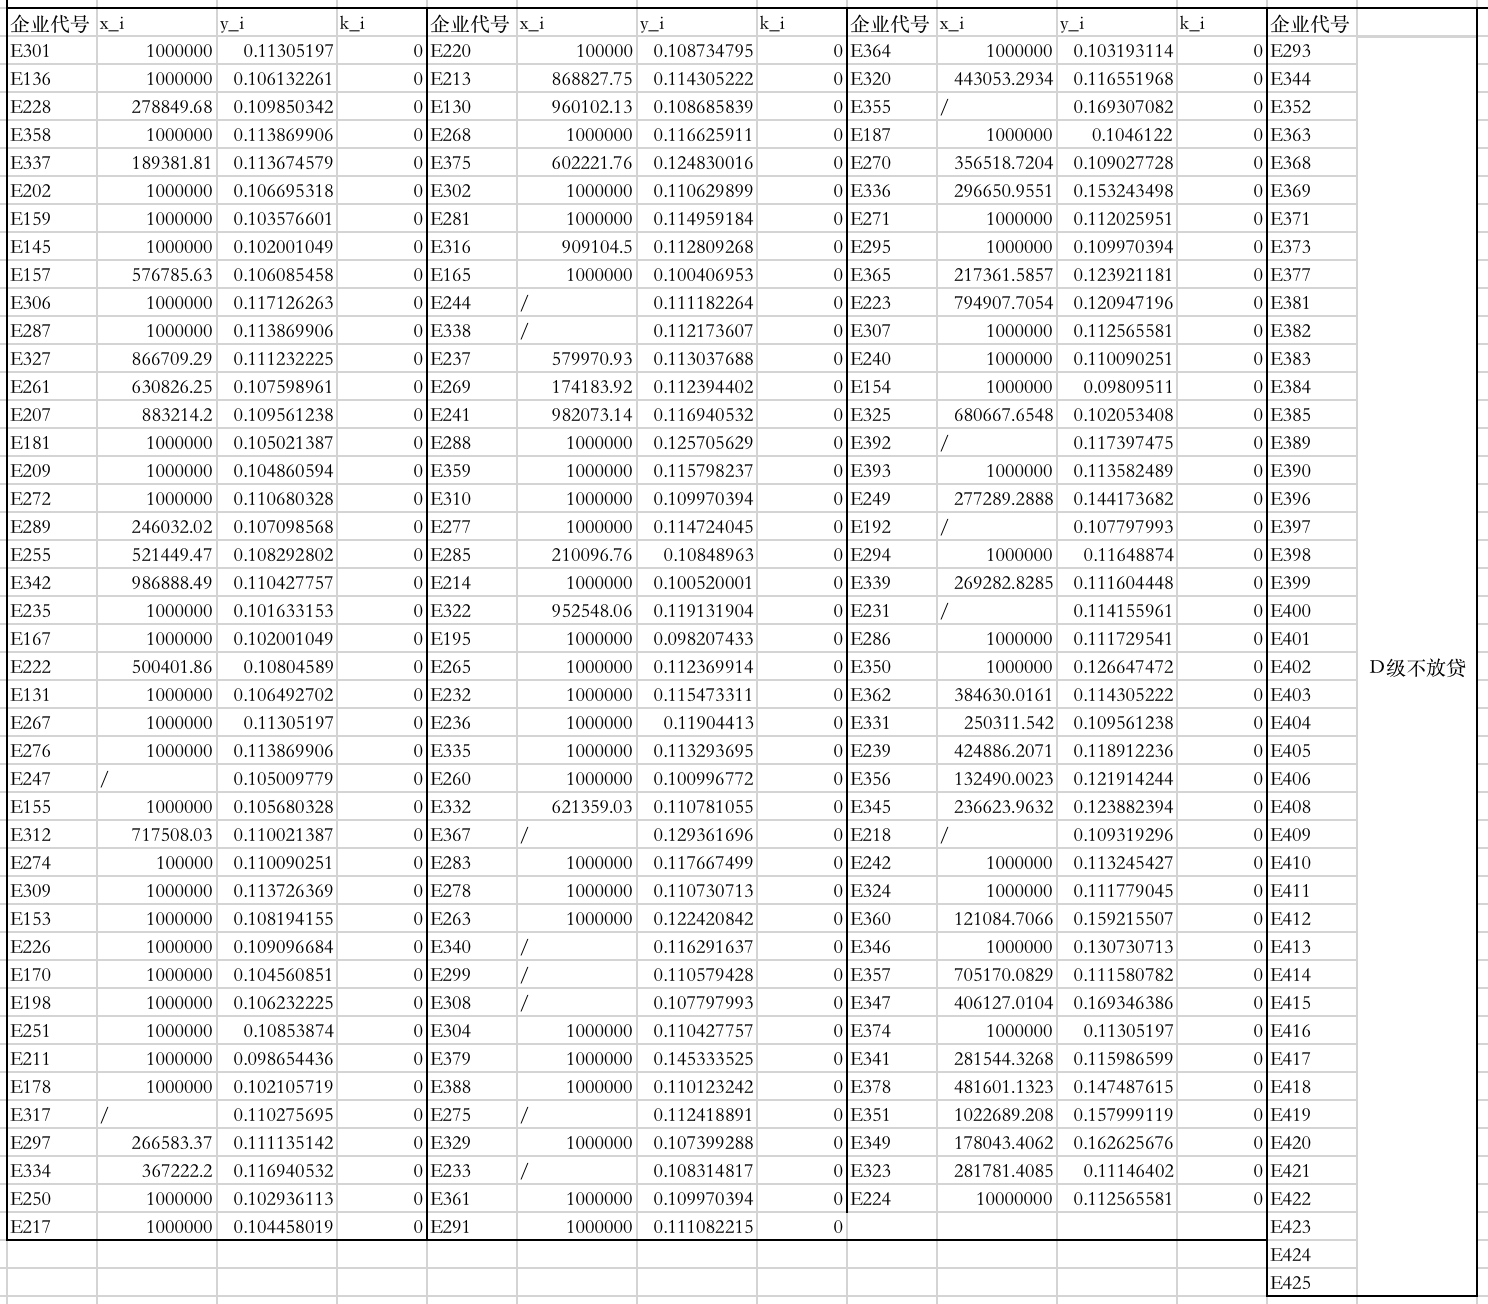
\includegraphics[width=1\linewidth]{figures/T2_2.jpg}  %插入的图,包括JPG,PNG,PDF,EPS等,放在源文件目录下
	\label{fig:mcmthesis-logo}   %标签,用作引用
\end{figure}



\newpage
 \noindent \textbf{附录七:对无信贷记录的302家企业在疫情因素下的投资决策}
 \begin{figure}[h]%%图	
	\centering  %插入的图片居中表示
	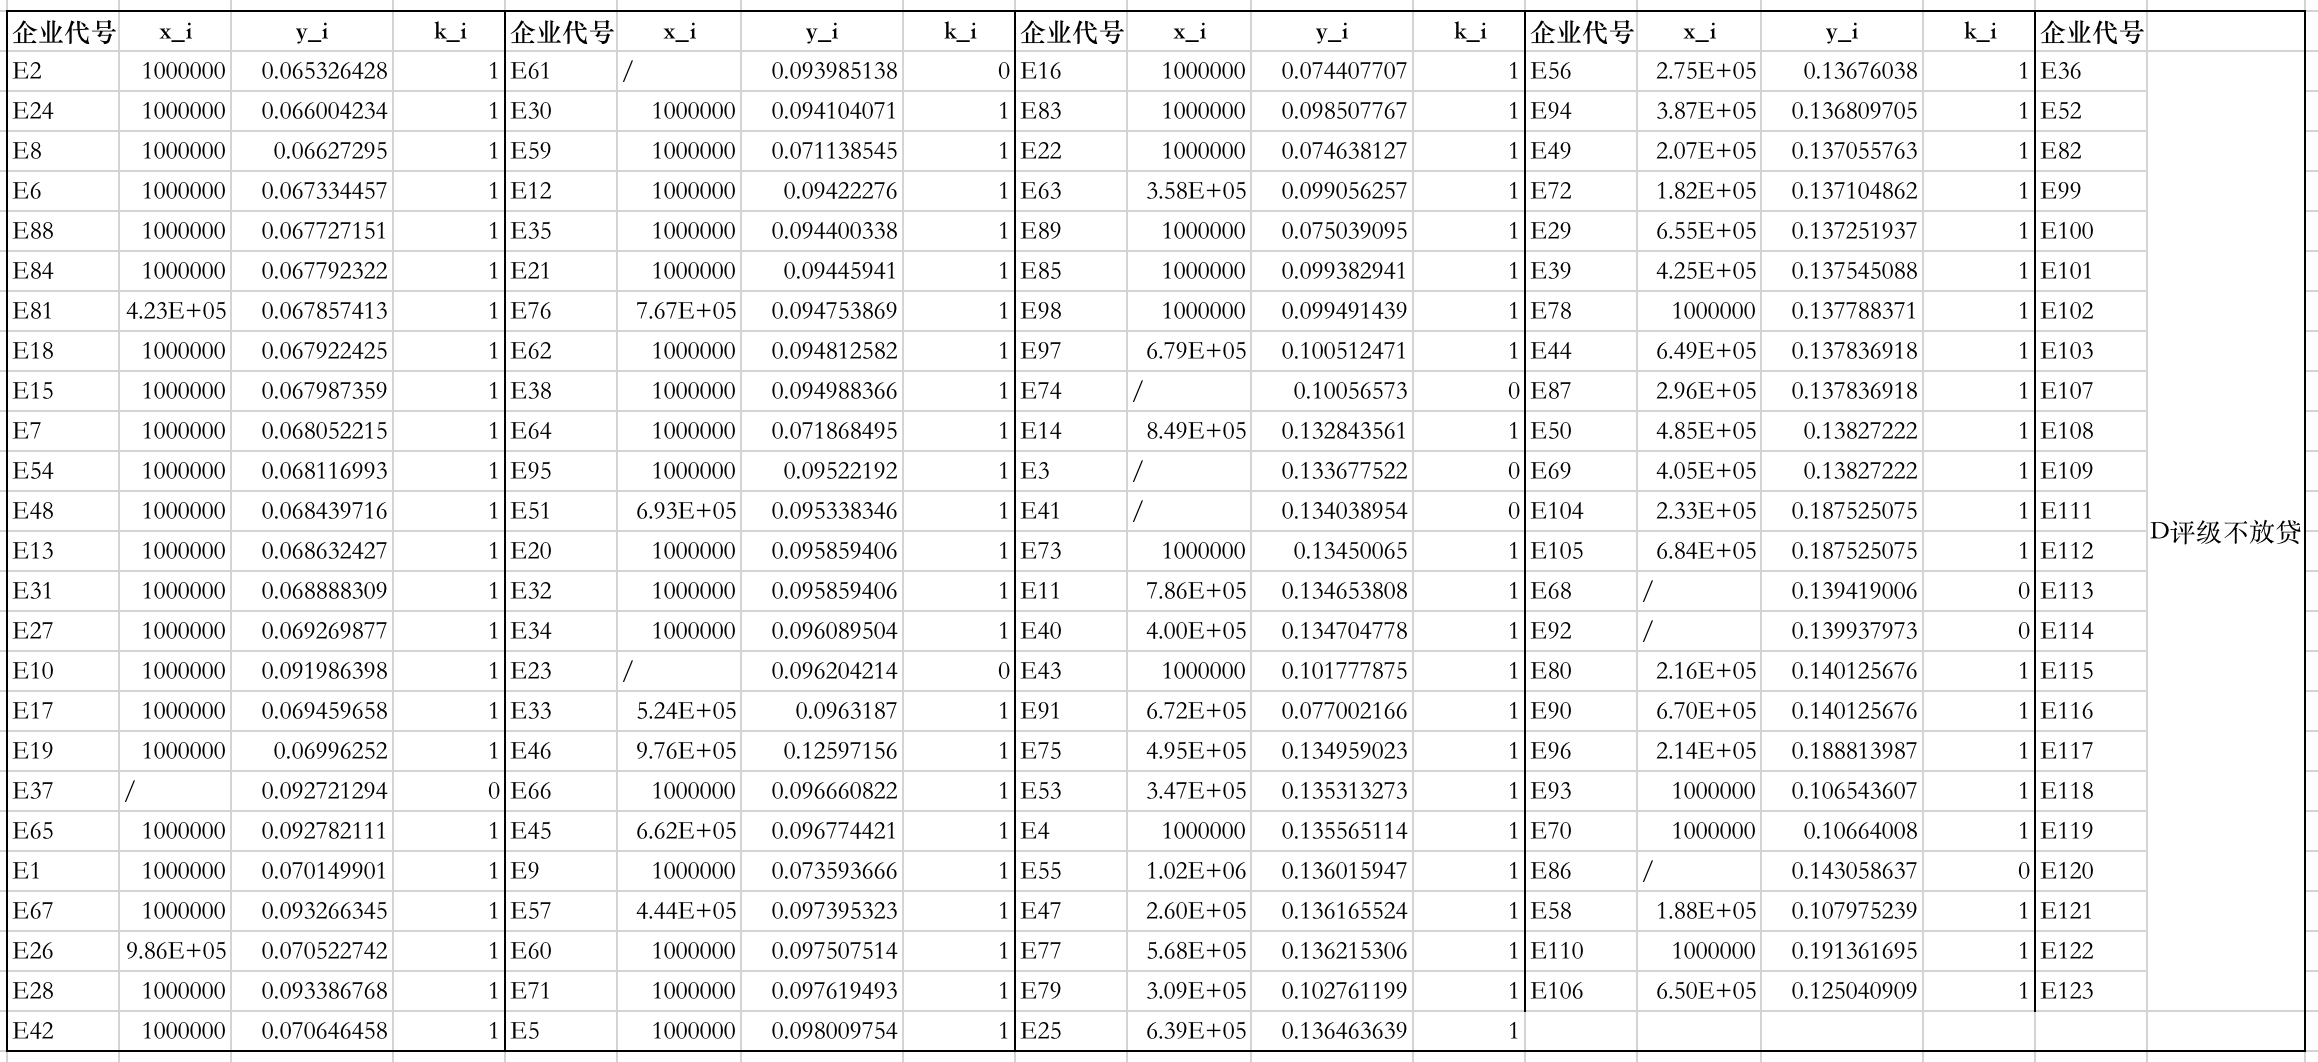
\includegraphics[width=1\linewidth]{figures/T3.jpg}  %插入的图,包括JPG,PNG,PDF,EPS等,放在源文件目录下
	\label{fig:mcmthesis-logo}   %标签,用作引用
\end{figure}
\end{appendices}

%\begin{figure}[!htb]
%   \centering
%\begin{tikzpicture}[font={\sf \small}]
%\def \smbwd{2cm}
%\thispagestyle{empty}

%定义流程图的具体形状
%\node (start) at (0,0) [draw, terminal,minimum width=\smbwd, minimum height=0.5cm] {原始数据};      % 定义开始
%\node (getdata1) at (0,-1.5) [draw, predproc, align=left,minimum width=\smbwd,minimum height=1cm] {数据预处理};
%\node (getdata2) at (0,-3.5) [draw, predproc, align=left,minimum width=\smbwd,minimum height=1cm] {特征提取};
%\coordinate (point3) at (0,-4.75);
%\node (getdata3) at (0,-5.5) [draw, predproc, align=left,minimum width=\smbwd,minimum height=1cm] {模型设计};
%定义预处理过程,读取数据
%\node (decide) at (0,-7.5) [draw, storage, minimum width=\smbwd, minimum height=1cm] {预测器};  %定义判断条件
%\node (storage) at (0,-9.5) [draw, storage, minimum width=\smbwd, minimum height=1cm] {比较器};     %定义数据存储
%\node (process) at (4,-7.5) [draw, process, minimum width=\smbwd, minimum height=1cm] {真实数据};      %定义处理过程
%\coordinate (point1) at (0,-10.75);
%\node (end) at (0,-11.75) [draw, terminal,minimum width=\smbwd,minimum height=0.5cm] {结束};        %定义结束

%连接定义的形状,绘制流程图--表示垂直线,|表示箭头方向
%\draw[->] (start) -- (getdata1);
%\draw[->] (getdata1) -- (getdata2);
%\draw[->] (getdata2) -- (getdata3);
%\draw[->] (getdata3) -- node[right]{$X_t$} (decide);
%\draw[->] (decide) -- node[right]{$X_t^{'}$} (storage);
%\draw[->] (decide) -- (storage);
%\draw[->] (point3) -| node[above]{$Y_t$} (process);
%\draw[->] (process) |- (storage);
%\draw[->] (storage) -- (end);

%\end{tikzpicture}
%\caption{模型结构}\label{fig:one}
%\end{figure}
 
\bibliographystyle{plain}
\bibliography{bibtex-example}
\newpage

\appendix


%\begin{lstlisting}
%\end{lstlisting}


\end{document}

